\documentclass[USenglish,oneside,twocolumn]{article}
\makeatletter

% Don't use the obsolete fixltx2e package on newer systems (2015 or later).
\@namedef{ver@fixltx2e.sty}{2006/03/24}
\@namedef{opt@fixltx2e.sty}{}

% Don't use the multicol package (it raises a warning in twocolumn format).
\@namedef{ver@multicol.sty}{2016/04/07}
\@namedef{opt@multicol.sty}{}

% Footnote hyperlinks don't work due to a conflict between hyperref and footmisc.
% Turning them off prevents the warnings and broken links.
\PassOptionsToPackage{hyperfootnotes=false}{hyperref}
\usepackage[utf8]{inputenc}%(only for the pdftex engine)
%\RequirePackage[no-math]{fontspec}%(only for the luatex or the xetex engine)


\usepackage[big]{dgruyter_NEW}


% Don't use non-existant fonts for labels in footnotes.
\def\@makefnmark{\hbox{\@textsuperscript{\normalfont\@thefnmark}}}
\makeatother
\usepackage[utf8]{inputenc}
\usepackage{hyperref}
\usepackage{subcaption}
\newtheorem{theorem}{Theorem}
%\usepackage{algorithmicx}
\usepackage{caption}
\usepackage{algorithm}
\usepackage[noend]{algpseudocode}
\algrenewcommand{\algorithmiccomment}[1]{{\color{gray}$\triangleright$ #1}}
\makeatletter
\def\plist@algorithm{\space}
\makeatother
\usepackage[
n,
advantage,
operators,
sets,
adversary,
landau,
probability,
notions,
logic,
ff,
mm,
primitives,
events,
complexity,
asymptotics,
keys
]{cryptocode}


\hyphenation{moneTor}
\hyphenation{CIRCWINDOWSTART}
\hyphenation{STREAMWINDOWSTART}
\makeatletter
\renewcommand{\ALG@beginalgorithmic}{\small}
\makeatother

\newcommand{\flo}[1]{ {\color{red} FR: #1}}
\newcommand{\td}[1]{ {\color{blue} TD: #1}}
\newcommand{\op}[1]{ {\color{olive} OP: #1}}

\cclogo{
\includegraphics{by-nc-nd.pdf}}
\begin{document}
 

\title{\huge Incentivizing Anonymous Communication with Efficient Nanopayment Channels} % TODO: replace with your title

\runningtitle{Monetary Tor Incentives with Efficient Nanopayment Channels}

  %\subtitle{...}
\begin{abstract}
{Tor, the most widely used and well-studied traffic anonymization network in
  the world, suffers from orthogonal limitations in network diversity and
  performance. We propose to mitigate both problems simultaneously through the
  introduction of a premium bandwidth market between clients and relays. To this
  end, we present moneTor: a relay incentivization scheme featuring anonymous,
  efficient, and economically robust nanopayments. Our approach leverages the
  latest advances in cryptocurrency research toward a design that is directly
  integrated into the existing Tor architecture. This work describes a
  full-stack strategy that covers economic policy, novel payment algorithms, and
  networking implementation. Through live empirical data collection and analysis
  of our emulated prototype, we argue that moneTor, based on short-lived channels on the top of a long-lived channel, is an elegant and
  feasible monetary incentive scheme for Tor, offering upwards of 100\%
  improvements in differentiated bandwidth for paying users at near-optimal
  throughput and latency overhead.}
\end{abstract}

  \keywords{Tor, cryptocurrency, payment channels}
%  \classification[PACS]{}
 % \communicated{...}
 % \dedication{...}

  \journalname{Proceedings on Privacy Enhancing Technologies}
\DOI{Editor to enter DOI}
  \startpage{1}
  \received{..}
  \revised{..}
  \accepted{..}

  \journalyear{..}
  \journalvolume{..}
  \journalissue{..}
  
  
 \maketitle


\section{Introduction}
\label{sec:introduction}
Anonymous traffic routing through Tor remains one of the most popular
low-latency methods for censorship evasion and privacy protection
~\cite{dingledine2004tor}. In this setup, clients protect their TCP/IP metadata
by routing their traffic through an onion encrypted path with three
randomly selected volunteer relay nodes, referred to as a circuit. The network
presently consists of $\approx 6,400$ relays contributing over 230 Gbit/s of
bandwidth globally~\cite{portal2018tormetrics}. While Tor has proven to be a
highly effective option for privacy-seeking users, it suffers from two
orthogonal issues that are relevant to this work. The first is the broad family
of collusion attacks. These threats are relevant in scenarios where an attacker,
who controls multiple nodes or network vantage points, is probabilistically placed at more than one hop
along a single circuit, opening a much easier path to client
deanonymization~\cite{wright2004predecessor,murdoch2005low}. The second
problem is overall performance. Although the overlay protocol itself generates
an inherent overhead in network resources, Tor suffers from additional traffic
congestion that leads to suboptimal network
performance~\cite{portal2018tormetrics, alsabah2016performance}.

One approach to mitigated these problems is to address them separately from a
networking standpoint. Indeed, a significant portion of recent research in Tor
proposes modifications to the core protocol itself, such as reengineering the
TCP+TLS part of the stack~\cite{reardon2009improving} or designing a better
kernel-aware scheduler~\cite{jansen2014never}. A second approach observes that
the anonymity and performance of the network are both proportional to the number
of nodes and users. From this perspective, the problem becomes a largely
economic question: how can we incentivize more relay participation? There is a
long line of research that explores various strategies for incentivization
spanning over the past decade. Progress in this field faces a multitude of
challenges. Consider the approach most relevant to our work: monetary
incentives. Aside from the analytically intractable set of legal and
sociopolitical obstacles, monetary payments in this environment must overcome a
trifecta of challenging constraints:

\begin{itemize}
\item \emph{Anonymity}: The paramount mission of Tor is user privacy. This
  cannot be compromised or reduced by transparent money transactions trail.
\item \emph{Payment Security}: Anonymity also prohibits the formation of large
  credit and trust systems. As such, financial transactions cannot transpire
  without strong guarantees of cryptographic security.
\item \emph{Efficiency}: Tor services millions of concurrent users, all of whom
  maintain largely short-term relationships. A robust payment system must handle
  extremely lightweight and scalable payments so as to accommodate the dynamic
  and often short-lived activities of these clients.
\end{itemize}

\textbf{Present Landscape} While a number of prior works satisfy some subset of
these constraints, no single proposal has thus far been sufficiently convincing
so as to warrant further development. We speculate that the lack of a
breakthrough in this niche area is not a matter of insufficient ingenuity but
rather one of timing. In recent years, there has been an explosion of academic
research within the domain of cryptocurrencies. As of this writing, Satoshi
Nakamoto's Bitcoin whitepaper has already garnered over 3,000 references in
citing publications~\cite{nakamoto2008bitcoin}\footnote{The recency of this
  development is highlighted by the fact that about half of this work is dated
  after 2017}. This body of work introduces a multitude of new concepts that
will prove indispensable to our own area of research. Our objective then, is to
leverage the full extent of these innovations into a practical next-generation
incentivization strategy for Tor.

\label{sec:Contributions}
\textbf{Contributions} The moneTor scheme is a novel full-stack framework for
Tor incentives. We make the following contributions in this paper:

\begin{enumerate}
\item Design an economic model to favor network diversity, offering enough
  market control such that the Tor project can decide which notion of diversity
  to promote
\item Introduce new highly-efficient nanopayment protocols which may be of some
  independent interest for other high-frequency payment applications
\item Specify an integration strategy to integrate payments and user incentives
  into the existing Tor architecture and networking layer
\item Collect privacy-preserving client usage data to justify design parameters
  and argue for efficacy
\item Implement a proof-of-concept partial prototype extending the Tor protocol
  in the core daemon, featuring more than 15k lines of code
\item Conduct network-scale simulations to analyzing the performance impact of
  our embedded payment and incentivization scheme
\end{enumerate}

The moneTor design leverages peer-reviewed research for some components and
novel, fully-specified techniques in all others. In effect, we claim that the
entire technical stack is accounted for and that moneTor can be feasibly
developed today.

\paragraph*{Roadmap.} In Section~\ref{sec:background}, we draw on technical preliminaries from two distinct fields: applied Tor research and payment channels. Section~\ref{sec:related_work} presents the related work. In Section~\ref{sec:economic} we describe how we engineer the flow of money in a way that is both economically stable yet still adheres to the core mission of the Tor project. In Section~\ref{sec:payment} we 
describe the technical construction for the moneTor payment scheme at the payment protocol level. We pursue in Section~\ref{sec:network} with the technical construction of moneTor at the network level. In section~\ref{sec:analysis} we  validate our design decisions with real-world data collection from live Tor users. 
In Section~\ref{sec:experimentations}, we validate our technical design via experiments performed on a proof-of-concept software implementation within the native Tor codebase. We finally address concerncs for limitations and future work in Section~\ref{sec:limitations_futurework} and conclude in Section~\ref{sec:conclusion}.

\section{Background}
\label{sec:background}
%\subsection{Tor}

%\paragraph*{Tor Architecture}
%The Tor network is composed of multiple different components, each of which run
%the same code base. Volunteers can run relays and enable specific roles or tasks
%such as \textit{network consensus directories}, \textit{HSDirs} and \textit{Exit
%  policies}. \textit{Directory authorities} and \textit{Bandwidth authorities}
%are the most important components of the network, and are only operated by
%trustworthy core contributors. There are currently nine directory authorities
%which periodically reach agreement over the state of the network, called the
%\textit{consensus document}. This consensus document holds the identification
%information related to all available relays inside the network, as well as the
%result of the authority vote (e.g., a set of \textit{flags} associated to each
%relay). The bandwidth authorities constantly measure every relay and provide to
%the directory authorities a measurement value for each of them, which plays a
%critical role in the path selection algorithm. This paper extends the
%architecture by adding two new roles needed for our monetary relay
%incentivization: $intermediary$ and $ledger$.

%\paragraph*{Traffic Analysis}
\textbf{Traffic Analysis.}
Tor's threat model assumes a local adversary who can observe some fraction of
the network and can operate or compromise a number of onion routers. Tor also
assumes a local adversary who can manipulate user streams by inserting,
modifying, deleting or delaying data to create observable perturbations.
Typically, by observing both ends of an anonymous stream, an attacker can infer
the participating parties using statistical correlation. The adversary's
precision can be further improved by adding traffic flow
perturbations~\cite{fu2009one}. This attack is called \textit{end-to-end
  correlation}. Tor does not implement explicit countermeasures to this attack
but does strive to minimize its impact. However, Rochet and Pereira recently
showed that Tor's essential forward-compatibility feature can be exploited in a
silent near-perfect and instantaneous active traffic confirmation
attack~\cite{rochet2018dropping}. These developments imply a serious need to
induce more diversity to the Tor network, which would make such traffic analysis
against a large fraction of Tor users more costly. One such solution is
presented in this paper.

% \paragraph*{Circuit handling on Tor clients}
\noindent
\textbf{Circuit handling on Tor clients.}
%
%\td{TODO: This section will provide a more detailed explanation of how circuits are
%created and how that affects moneTor's high initial latency and overhead design}
The key element of the Tor protocol is the Tor circuit, which is a randomly
constructed 3-hop routing path through the overlay network. Within a circuit,
Tor multiplexes one or more streams to handle application traffic. In order to
reduce latency in the user experience, Tor attempts to build circuits
preemptively as soon as the client obtains the necessary directory information.
Once a stream is created by a user application, it can be immediately routed
through the idle circuit, dramatically improving latency. The anticipated number
of required preemptive circuits is dynamically calculated every second by the
Tor client. We exploit this same strategy for moneTor's circuit channel setup
routine by building preemptive payment channels and show that it too can
dramatically improve the time to first payment.

%\paragraph*{Evaluating Tor's performance}
%Shadow~\cite{jansen2011shadow} is a discrete event networking simulator that
%allows real, unmodified applications to run within a virtual network. Its
%primary advantage is the ability to run native networking application code that
%interfaces with the simulator via an external application-specific
%plugin. Within the simulation environment itself, Shadow faithfully mimics the
%real Tor network conditions including bandwidth and latency. As a result,
%experiments conducted with this tool tends to be more accurate than ones
%conducted over alternatives such as private university networks or
%PlanetLab~\cite{chun2003planetlab}. We utilize the shadow framework to
%evaluate the costs and performance of our algorithms over network-level
%simulations.

%\subsubsection{Tor's Scheduling}

%\paragraph*{Flow Control}

\noindent\textbf{Flow Control}
Tor seeks to maintain an optimal flow of cells in
each circuit by capping the rate of transmission to fixed-sized windows.
%The
%CIRCWINDOWSTART value dictates flow for the overall circuit while
%STREAMWINDOWSTART dictates each end-to-end flow between a client and the edge
%connection at an exit relay.\footnote{Default values, expressed in number of
% cells, are CIRCWINDOWSTART = 1000 and STREAMWINDOWSTART = 500.}
%The number of
%cells going in each direction are tracked separately.
In effect, the protocol attempts to keep the flow of cells on each circuit as
full as possible while ensuring fairness between streams and that the number of
cells in transition do not exceed a limit default of 1000. Flow control has a
strong impact on network conditions as shown by AlSabah \textit{et
  al.}~\cite{pets2011-defenestrator} in work toward improving total global
performance. In the design of moneTor, we will adapt these flow control windows
toward our somewhat different objective to prioritize paid traffic.

%\paragraph*{Payment Channels}



%\textbf{Secure Payments} The modern generation of decentralized digital
%currencies traces its roots to Nakamoto's Bitcoin
%protocol~\cite{nakamoto2008bitcoin}. This family of payment protocols is
%characterized by use of a public distributed ledger, often a blockchain, and a
%notion of identities and ownership based in public key cryptography. A wide
%range of base-layer payment protocols have emerged; most relevant for our
%purposes is the fully programmable smart contract platform
%Ethereum~\cite{wood2014ethereum} and anonymity-focused schemes such as
%Zerocash~\cite{sasson2014zerocash} and Cryptonote~\cite{van2013cryptonote}. In
%this second class of anonymous currencies, the general security model requires
%that the payment sender is able to upload verifiable and irreversible proof of
%payment to the ledger without leaking sender identity, recipient identity, or
%payment value. Cryptonote achieves a probabilistic guarantee of privacy using a
%combination of lightweight ring signatures and stealth addresses but may be
%vulnerable in typical use~\cite{miller2017empirical}. Zerocash achieves stronger
%theoretical anonymity by leveraging more expensive non-interactive
%zero-knowledge proofs which require a trusted setup phase.
%
%Researchers have explored interoperability between ledgers . Back et al.\
%published the first primitive proposal for \emph{sidechains}, which
%conceptualizes a secondary blockchain ledger that can send and receive assets
%from the primary Bitcoin blockchain~\cite{back2014enabling}. More recently, Poon
%and Buterin explain how Ethereum can support multiple levels of arbitrarily
%configured \emph{child chains} that inherit many security properties from the
%original blochain.

\noindent\textbf{Payment Channels.}
The core cryptocurrency component featured in moneTor is the tripartite
bidirectional micropayment channel. Base layer cryptocurrency protocols are
typically capped on the order of tens of transactions per
seconds~\cite{team2018blockchain}. The most actively pursued path toward better
scalability thus far is work in off-chain payment channel networks popularly
known as ``Lightning Networks''~\cite{poon2016bitcoin}. In this setup, a single
ledger transaction is used to escrow funds by two parties $A$ and $B$. These
parties may then proceed to make bidirectional micropayments to each other
\emph{without ledger interaction} through the exchange of signed ``I Owe You''
tokens. By themselves, channels are useful for reducing the number of ledger
interactions for parties with reoccurring interactions. More consequential for
the scalability problem is the tripartite channel paradigm in which $A$ pays $B$
through some \emph{intermediary} party $I$ with which they both maintain active
channels. In practice, $A$ and $B$ might occupy the roles of a customer and
merchant who are registered with a well-known financial service provider $I$.
$A$, $B$, and $I$ need only interact with the ledger periodically to deposit and
withdraw large sums of money, improving the network capacity by multiple orders
of magnitude. Informally, tripartite channels are secure if the following
requirements are met.

\begin{enumerate}
\item At every step of the protocol, all parties possess proof of execution of
  the last finalized payment state
\item Given two proofs of payment state, the network can unambiguously identify
  the more recent state.
\item When $A$ agrees to pay $B$ through $I$, the payment is atomic. That is,
  there is never a situation in which $I$ pays $B$ but is unable to extract the
  agreed-upon payment from $A$.
\end{enumerate}

%The guarantees are achieved in the Bitcoin Lightning network and other similar
%protocols through simple hash commitment and transaction delay primitives. The
%end result is a game-theoretic notion of security whereby all parties are
%incentivized to behave honestly.

 The micropayment channel concept has since been extended to support anonymity
 design goals. Tumblebit is a channel-like mixing protocol designed for Bitcoin
 that allows fast and anonymous off-chain payments~\cite{heilman2017tumblebit}.
 Malvavolta~\textit{et al.}~\cite{malavolta2017concurrency} describe a variant on
 payment channels that provides Tor-like privacy in the sense that
 sender/receiver privacy is preserved under the assumption of at least one
 trusted intermediary. However, these schemes are not ideal for our purposes as
 Tumblebit requires unrealistic synchronization between payment parties for the
 Tor environment while Malvavolta~\textit{et al.} introduces additional
 potentially malicious parties.

 We show in Section~\ref{sec:payment_overview} how an extension to
 Bolt~\cite{green2017bolt}, a tripartite anonymous channel protocol based on
 zero-knowledge proofs proposed by Green and Miers, is applicable to Tor
 incentives while providing technical guarantees of anonymity, efficiency, and
 payment security. This framework defines the anonymity set with respect to the
 collection of users connected to the same intermediary. In other words, given a
 set of end users $E_{all} = \{E_1, E_2, ... E_n\}$ who each have an active
 channel with $I$, $E_a$ should be able to send a secure payment to $E_b$ such
 that $I$ cannot identify $E_a$ or $E_b$ from $E_{all}$ nor can $I$ infer the
 payment value. Of course, $I$ must still be able to verify that the payment is
 valid and that its internal channel states have been updated accordingly.

%\paragraph*{Anonymous Payment Channels} The micropayment channel concept has
%since been extended to support anonymity design goals. In particular, the
%moneTor builds on the work of Bolt, a tripartite anonymous channel protocol
%based on zero-knowledge proofs proposed by Green and Miers~\cite{green2017bolt}.
%This framework defines the anonymity set with respect to the collection of users
%connected to the same intermediary. In other words, given a set of end users
%$E_{all} = \{E_1, E_2, ... E_n\}$ who each have an active channel with $I$,
%$E_a$ should be able to send a secure payment to $E_b$ such that $I$ cannot
%identify $E_a$ or $E_b$ from $E_{all}$ nor can $I$ infer the payment value. Of
%course, $I$ must still be able to verify that the payment is valid and that its
%internal channel states have been updated accordingly. Several nuances arise
%concerning end user privacy in certain situations, such as during the
%micropayment setup escrow phase and in the event that $I$ maliciously aborts. We
%do not consider it necessary to discuss these caveats here as they are not
%prohibitively problematic for our later treatment of anonymous payment channels.

%In our review of the existing literature, we assessed that the anonymous
%tripartite payment channel paradigm uniquely provides the trustless, scalable
%infrastructure necessary to satisfy our constraints. However, for completeness,
%it is worth enumerating other options we considered. Tumblebit is a mixing
%protocol designed for Bitcoin that allows fast and anonymous off-chain payments
%but requires an infeasible synchronization procedure between payment
%parties~\cite{heilman2017tumblebit}. Malvavolta et\ al.\ describe a variant on
%payment channels that provides Tor-like onion-routing privacy along the payment
%path~\cite{malavolta2017concurrency}. However, implementation into Tor would
%require the network to either A) force relays to process payment channels or B)
%introduce more potential malicious parties along the payment route. Bipartite
%payment channels~\cite{zhang2019z} suffer from the same centralized scalability
%concerns discussed in Section~\ref{sec:related_work}. Finally, probabilistic
%payments, if sufficiently anonymized, imposes costly cryptographic operations at
%client endpoint~\cite{chiesa2017decentralized}.

%The micropayment channel concept has since been extended to support anonymity
%design goals. Tumblebit is a channel-like mixing protocol designed for Bitcoin
%that allows fast and anonymous off-chain payments~\cite{heilman2017tumblebit}.
%Malvavolta~\textit{et al.}~\cite{malavolta2017concurrency} describe a variant on
%payment channels that provides Tor-like privacy in the sense that
%sender/receiver privacy is preserved under the assumption of at least one
%trusted intermediary. However, these schemes are not ideal for our purposes as
%Tumblebit requires unrealistic synchronization between payment parties for the
%Tor environment while Malvavolta~\textit{et al.} introduces additional
%potentially malicious parties.

%We show in Section~\ref{sec:payment_overview} how well an extension to
%Bolt~\cite{green2017bolt}, a tripartite anonymous channel protocol based on
%zero-knowledge proofs proposed by Green and Miers, is applicable for Tor
%incentives and provides the technical promise of anonymity, efficiency and
%payment security.
%%Our construction called moneTor bridges the theoretical advance in the
%%cryptocurrency space with the concrete requirements of a complex and advanced
%distributed system such as the Tor network.
%One of the reasons that influence our choice of Bolt as a starting point is the
%potential that we saw in designing and building a payment system that shifts
%away the heavy cryptography from the critical path when performing payments
%(i.e., when exchanging data, the cost of processing payments is reduced to only
%one hash operation with moneTor).

%\paragraph*{Anonymous Payment Channels} The micropayment channel concept has
%since been extended to support anonymity design goals. Tumblebit is a
%channel-like mixing protocol designed for Bitcoin that allows fast and
%anonymous off-chain payments~\cite{heilman2017tumblebit}. Malvavolta
%et\ al.\ describe a varient on payment channels that provides Tor-like
%privacy in the sense that sender/receiver privacy is preserved under
%the assumption of at least one trusted
%intermediary~\cite{malavolta2017concurrency}. However, these schemes
%are not ideal for our purposes as~\cite{heilman2017tumblebit} requires
%unrealistic synchronization between payment parties for the Tor
%environment while~\cite{malavolta2017concurrency} introduces
%additional potentially malicious parties. More applicable is Bolt, a
%tripartite anonymous channel protocol based on zero-knowledge proofs
%proposed by Green and Miers~\cite{green2017bolt}. In this framework,
%the anonymity set is defined with respect to the collection of users
%connected to the same intermediary. In other words, given a set of end
%users $E_{all} = \{E_1, E_2, ... E_n\}$ who each have an active
%channel with $I$, $E_a$ should be able to send a secure payment to
%$E_b$ such that $I$ cannot identify $E_a$ or $E_b$ from $E_{all}$ nor
%can $I$ infer the payment value. Of course, $I$ must still be able to
%verify that the payment is valid and that its internal channel states
%have been updated accordingly. Several nuances arise concerning end
%user privacy in certain situations, such as during the micropayment
%setup escrow phase and in the event that $I$ maliciously aborts. We do
%not consider it necessary to discuss these caveats here as they are
%not prohibitively problematic for our later treatment of anonymous
%payment channels.



%%% Local Variables:
%%% mode: latex
%%% TeX-master: "../popets_monetor"
%%% End:


%
%\section{Economic Design}
%\label{sec:economic}
%
We first summarize the economic layer of the incentivization scheme. At this
level, we assume the existence of an ideally secure and efficient payment layer
and proceed to outline the high-level policy design. The challenge here is to
engineer the flow of money in a way that is both economically stable yet still
adheres to the core mission of the Tor Project.

\subsection{Economic Policy}
The moneTor scheme allows for relays to offer a \emph{premium bandwidth} product
to Tor users in exchange for monetary payments. Under this framework,
financially willing users send payments directly to each relay along their circuits
in exchange for higher internet bandwidth and faster download speeds relative to
unpaid users. % The moneTor tokens themselves can be viewed as wrappers for some
% external financial asset that is converted at an exchange service.
The moneTor tokens %assets
may be any form of programmatic money which satisfies the standard properties of
\textit{scarcity}, \textit{fungibility}, \textit{divisibility},
\textit{durability}, and
\textit{transferability}~\cite[p.3]{crump2011phenomenon} A schematic of the cash
flow cycle is illustrated in Figure~\ref{fig:economic}.

\begin{figure}[h] \centering
  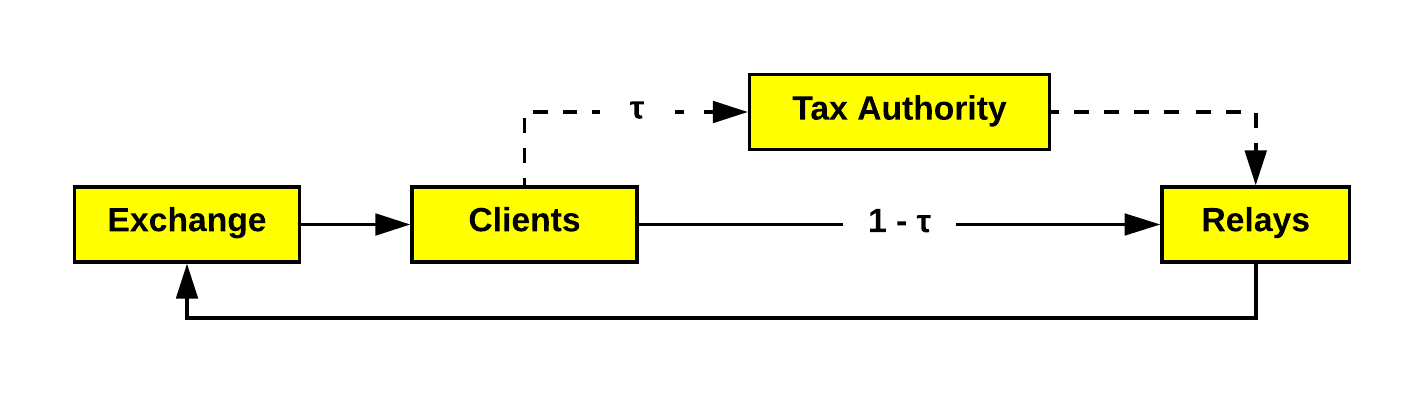
\includegraphics[trim={0.5cm, 0.5cm, 0.5cm, 0.5cm}, clip, scale=0.7]{images/economic_diagram.png}
  \caption[Cash Flow]{Cash Flow --- movement of moneTor tokens through the
    network. The value $\tau$ denotes the fraction of money that is collected
    for taxation purposes.}
  \label{fig:economic}
\end{figure}


We introduce a novel concept within the field in the form of a
taxation element. Intuitively, the shape of the network that will
emerge in a purely profit-seeking environment may not perfectly
correspond with the central goals of the Tor Project. The Tor Project
may for instance desire to compensate certain types of relays more
than others in order to improve the overall quality of the network
(e.g., supporting areas where anonymity is particularly important but
financial resources scarce). To this end, we accommodate for a stream
of taxed income that is anonymously diverted into a shared pool of
funds. These funds are selectively redistributed to relays via a
transparent policy.  In essence, taxation provides a tunable control
mechanism for The Tor Project to shape the topology of the network
towards some notion of optimal diversity and performance. The exact
content of such policy is an active subject of research that is
orthogonal to our paper (e.g., Waterfilling~\cite{waterfilling-pets2017} argues for security by maximum diversity in endpoints of user paths, and TAPS~\cite{taps-ndss2017} argues for security by trust policies). 

A key economic question to address is the issue of price determination. While it
would be tempting to enlist some market-based mechanisms to set premium
bandwidth prices, any price differentiation between clients or relays inevitably
leaks more information. This leakage becomes more severe with higher granularity
payment options as adversaries begin to use price to link payment channels and
circuits. We therefore impose the constraint that all users should pay a single
uniform price for premium bandwidth at any time $t$. This price may be set
through a centralized calculation by the authorities or a more dynamical
consensus vote reached by the network.

The payment system we present in the next Section~\ref{sec:payment} is independent of the token creation for which multiple strategies are available. For example, the moneTor tokens could be viewed as wrappers for some external financial asset that is converted at an exchange service with an 1-to-1 mapping. In this scenario, moneTor tokens are created when the users buy them with other coins and destroyed when the users sell them for other coins.  A second example would be to let the Tor project creates and destroys moneTor tokens at will. In such scenario, the directory authorities handle the tokens as a resource management system, but do not trade them against fiat currencies or other coins. Given the transferability of the moneTor tokens, we would expect a side-market to appear for which the Tor project would not be responsible. These two approaches have both advantages and inconveniences usually linked to political opinions and ideologies.

\subsection{Incentivized Conformity} In a decentralized network, there is no
practical way to enforce standard behavior at each local node. We must therefore
consider whether all nodes are rationally incentivized to obey the stipulated
policies. For instance, we cannot guarantee that relays will actually confer
premium bandwidth to paying users. Even though the relay has no particular
reason to deviate, the client should periodically monitor her bandwidth and only
make payments when they appear to be making a difference. The relationship
between the client and relay can then be modelled as a game theoretic tit-for-tat
dynamic.

At the opposite end of the spectrum, relays might overly prioritize premium
circuits while rejecting all traffic from unpaid users. They might also attempt
to game the tax redistribution process to gain larger share of the proceeds. The
bandwidth measurement authorities must anticipate such modes of deviation from
the standard behavior to ensure that the risk for a relay to get blacklisted
from the network is greater than the incremental gains it might attain from
cheating. These attacks, while manageable, suggest that it would be prudent to
limit the complexity of our economic policies until we can better study
behavioral deviation dynamics in the live network.

%%% Local Variables:
%%% mode: latex
%%% TeX-master: "../main"
%%% End:


\section{Payment Design}
\label{sec:payment}
%Where we previously assumed the existence of an ideal payment procedure, we now
%describe the concrete technical construction for the moneTor payment scheme.

\subsection{Economic considerations}

% A schematic of the cash
%flow cycle is illustrated in Figure~\ref{fig:economic}.

%\begin{figure}[h] \centering
%  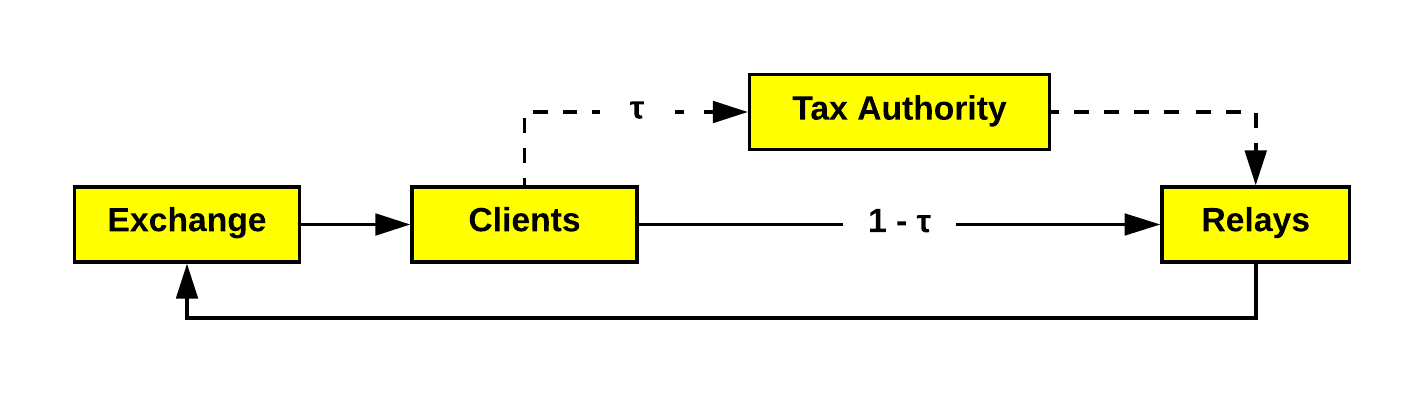
\includegraphics[trim={0.5cm, 0.5cm, 0.5cm, 0.5cm}, clip, scale=0.7]{images/economic_diagram.png}
%  \caption[Cash Flow]{Cash Flow --- movement of moneTor tokens through the
%    network. The value $\tau$ denotes the fraction of money that is collected
%    for taxation purposes.}
%  \label{fig:economic}
%\end{figure}

Given the delicate nature of this research area, a key motivation in
the design of our scheme is to explicitly accommodate some of the more
consequential economic considerations. For instance, to ensure that
tokens maintain real-world value, the Tor Project has two 
choices. One option is to reserve total monetary policy, allowing
moneTor tokens to mirror some external value signal such as the USD or
the Euro. Alternatively, by making use of such inter-ledger protocols~\cite{back2014enabling}~\cite{poon2017plasma}, tokens can act
as wrapper for an external cryptocurrency such as Bitcoin or
Ethereum. This choice represents a tradeoff between financial
stability and responsibility and our technical scheme allows for
either option.

The shape of the network that will emerge in a purely profit-seeking
environment may not perfectly correspond with the central goals of the
Tor Project: to advance human rights and freedoms. To this end, we
introduce a taxation element, enabling a tunable control mechanism
for The Tor Project to shape the topology of the network towards some
notion of desirable diversity and performance. Taxes in moneTor are
anonymously diverted into a shared global fund and eventually
redistributed to relays via a transparent policy, for instance, to
support areas where anonymity is needed but financial resources are
scarce. The exact content of such policy is an active subject of
research that is orthogonal to our paper.~\footnote{E.g.,
  Waterfilling~\cite{waterfilling-pets2017} argues for security by
  maximum diversity in endpoints of user paths, and
  TAPS~\cite{taps-ndss2017} argues for security by trust policies.}

The final consideration is the issue of price determination. While it
would be tempting to enlist some market-based mechanisms to set premium
bandwidth prices, any price differentiation between clients or relays inevitably
leaks more information. This leakage becomes more severe with higher granularity
payment options as adversaries begin to use price to link payment channels and
circuits. We therefore impose the constraint that all users should pay a single
uniform price for premium bandwidth at any time $t$. 

%This price may be set
%through a centralized calculation by the authorities or a more dynamical
%consensus vote reached by the network.



%\subsection{Incentivized Conformity} In a decentralized network, there is no
%practical way to enforce standard behavior at each local node. We must therefore
%consider whether all nodes are rationally incentivized to obey the stipulated
%policies. For instance, we cannot guarantee that relays will actually confer
%premium bandwidth to paying users. Even though the relay has no particular
%reason to deviate, the client should periodically monitor her bandwidth and only
%make payments when they appear to be making a difference. The relationship
%between the client and relay can then be modeled as a game theoretic tit-for-tat
%dynamic within the immediate session. Over the long term, non-conforming relays
%might be blacklisted via Tor's existing reporting system.
%
%At the opposite end of the spectrum, relays might overly prioritize premium
%circuits while rejecting all traffic from unpaid users. They might also attempt
%to game the tax redistribution process to gain larger share of the proceeds. The
%bandwidth measurement authorities must anticipate such modes of deviation from
%the standard behavior to ensure that the risk for a relay to get blacklisted
%from the network is greater than the incremental gains it might attain from
%cheating. These attacks, while manageable, suggest that it would be prudent to
%limit the complexity of our economic policies until we can better study
%behavioral deviation dynamics in the live network.


\subsection{Ledger}

%The moneTor framework first requires a base layer payment protocol for users to
%anonymously and securely manage their funds.
In our payment design, we follow the Bitcoin paradigm in which all users
maintain full and exclusive control of their monetary wealth through use of
public key cryptography~\cite{nakamoto2008bitcoin}. However, unlike Bitcoin, it
is unnecessary for moneTor to rely on an inefficient decentralized consensus
mechanism. Since Tor already relies on a centralized set of authorities, we
simply introduce a new ledger authority role to maintain the global payment
state on a public tamper-evident database~\cite{crosby2009efficient}. To
maximize availability, this ledger may also be distributed across several
authorities with, for example, the architecture proposed by
RSCoin~\cite{danezis2015centrally}. This work focuses on payment protocol designs and evaluation. Therefore, we consider the investigation and choice of the right ledger technology as an independent problem out of scope of this paper.

%\op{Maybe add that RScoin might be a good ledger architecture on which our protocols rely?}

%%%
%  This part would either need more information or be removed to avoid reviewers to feel confused
%%%
%Structuring the ledger to understand
%blockchain-like semantics allows us to make use of recent developments in
%blockchain interoperability, allowing moneTor tokens to be pegged at a 1:1 ratio
%to a more popular cryptocurrency such as Bitcoin or
%Ethereum~\cite{back2014enabling, poon2017plasma}. The Plasma model in particular
%has many desirable properties. Under this setup, the moneTor ledger would act as
%a ``child chain'' that is coupled to the main Ethereum blockchain. This allows
%the external public blockchain to become the authority ledger of last resort in
%the event that the moneTor ledger goes offline. Effectively, honest users will
%always be able to make some claim to their funds so long as the Ethereum network
%is operational.
%Finally, moneTor requires anonymous payment procedures to allow users to make
%private low-frequency transactions. Potential candidates include Cryptonote,
%which makes use of stealth addresses and ring
%signatures~\cite{van2013cryptonote}, and Zerocash, which employs more expensive
%but more theoretically secure zero-knowledge proofs~\cite{sasson2014zerocash}.

\subsection{Payment Protocols Overview}
\label{sec:payment_overview}

In this section we specify formal protocols that comprise the payment
scheme. All protocols are either two or three party interactions between a
subset of the following roles: $C$ (client), $R$ (relay), $E$ (end user: either
a client or relay), $I$ (intermediary), and $L$ (ledger). All communications between end users and Intermediaries or the ledger are routed through Tor circuits.

The moneTor payment scheme is an extension of Bolt's three-party
bidirectional micropayment channels. In Bolt, multiple payments happens off-chain and cannot be linked together, even if the parties collide. Inspired from the Lightning Network~\cite{poon2016bitcoin}, payments can be routed through a third-party in a trustless fashion. In our design, we introduce an Intermediary relay which is only tasked to provide \emph{atomic} payment channel services between clients and relays and does not participate in routing user streams. These choices are argued from the following benefits: 1) it escapes the naive setting whereby each Tor client maintains a micropayment channel with each
relay would incur an $O(n*m)$ cost with
respect to channel management complexity, with $n$ the number of Tor clients and $m$ the number of relays. By engineering an additional
intermediary layer, the complexity of moneTor channel connections is
reduced to $O(n+m)$; 2) CPU-intensive tasks are shifted by our protocol design to those intermediaries, allowing a payment system far more efficient than previous work in critical positions (i.e., relays, Tor authorities and clients). We detail it in related work Section~\ref{sec:related_work}; 3) the intermediaries can be incrementally deployed to match the right trade-off between performance of channel establishments and partition of premium users anonymity set (i.e., typically a premium user uses a same intermediary during a long time, we will see why later).
We adopt Bolt's nomenclature where
possible but adapt it to our concepts of ledgers, clients, and relays. The
following is brief outline of the prerequisite micropayment channel procedures
defined in Bolt. We refer the reader to the original paper for more detailed
specifications~\cite{green2017bolt}.

\begin{itemize}
\item \textbf{KeyGen}: Any party generates a cryptographic keypair
\item \textbf{Init-E}: $E$ initializes half of a micropayment channel by
  escrowing funds on $L$
\item \textbf{Init-I}: $I$ initializes half of a micropayment channel by
  escrowing funds on $L$
\item \textbf{Establish}: $E$ and $I$ interact to establish a new micropayment
  channel from their respective halves
\item \textbf{Pay}: $C$ interacts with $I$ and $R$ to send a single micropayment to $R$
\item \textbf{Refund}: $E$ closes a channel on $L$ and makes a claim on
  the escrowed funds.
\item \textbf{Refute}: $I$ closes a channel on $L$ and makes a claim on
  the escrowed funds.
\item \textbf{Resolve}: $L$ determines the final balance of funds awarded to
  each party.
\end{itemize}

Bolt's micropayment channels suffer from relatively heavy cryptography ($37-100\ ms$) and communication
(7 message legs)~\cite{green2017bolt} is a prohibitive expense for Tor relay payments. Indeed, using Bolt would not permit a fair exchange (i.e., a high payment rate) between a client and a relay since we would need several \textit{RTTs} to complete a payment while ``consuming'' premium bandwidth and not being able to keep up with payments (in Bolt, the previous Pay needs to be finished to start the next one). Moreover, in terms of CPU overhead, it is also desirable to keep the
barrier of entry low for smaller relay operators. To overcome these
concerns, we present a new payment layer design enabling far more efficient
nanopayments that will satisfy our fair exchange problem and our overhead problem.

\textbf{moneTor} The moneTor construction makes use of the existing anonoymous
micropayment structure to build \emph{locally transparent nanopayments}. In
this scheme, \emph{nanopayment channels} between clients and relays are established in place of a single
micropayment operation through an intermediary (Figure~\ref{fig:parties}). These lightweight channels allow the client to send $n$
number of unidirectional nanopayments to the relay. Each payment represents a
fixed value $\delta$, established at the start of the channel. The payments
themselves are \emph{locally transparent} in the sense that each nanopayment in
the same channel is trivially linked to each other (in contrast to previous works where several payments in the same circuit were needlessly unlinkable from relay's viewpoint, details in Section~\ref{sec:related_work}). However, the nanopayment
channels themselves are unlinkable to other nanopayment channels and
micropayment operations. It is by design that this channel anonymity model fits
well with Tor's existing circuit framework in which one nanopayment channel is attached per circuit for each relay, and in which messages within circuits are
linkable with each other but the circuits themselves are not. In this sense, the
overarching motivation of our work is to relax the costly anonymity guarantees
provided by Bolt toward the design of a new set of protocols that have been
optimized for Tor. Note that the establishments and closures of nanopayment channels do not require the clients or relay to interact with the ledger, which offers a far more scalable design than previous works as we do not need to scale trusted or semi-trusted entities (only trustless intermediaries).

 We now briefly describe our new set of protocols.
\begin{figure}[h] \centering
  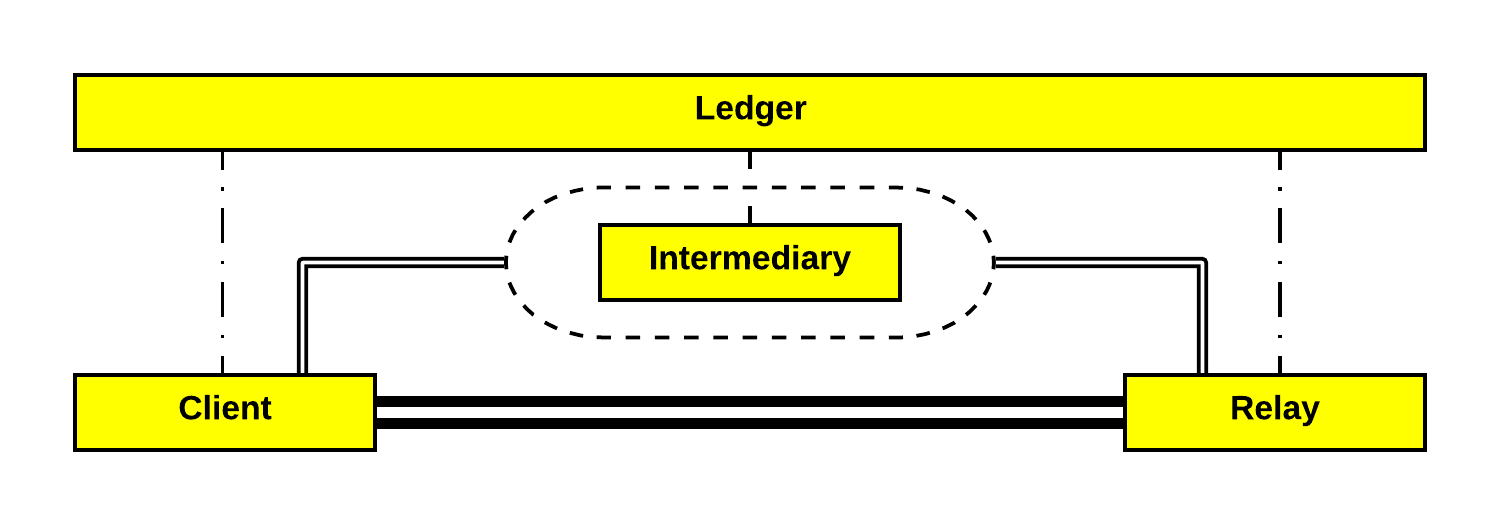
\includegraphics[trim={0.5cm, 0.5cm, 0.5cm, 0.5cm}, clip, scale=0.6]{images/party_diagram.png}
  \caption[Payment Roles]{Payment Roles --- Dashed lines represent periodic
    transactions (rare), thin double lines indicate micropayment channels (used at the beginning and end of circuits lifetime), and thick
    double lines indicate a nanopayment channel (handling nanopayments during the lifetime of the circuit). The dashed outline around the
    intermediary represents a notion of payment anonymity for the end users. Connections to the ledger and to the intermediary are protected by an internal Tor circuit.}
  \label{fig:parties}
\end{figure}
Any two parties $C$ and $R$ can construct a nanopayment channel once both have
completed Bolt $Establish$ with a common intermediary $I$. We define the following
set of protocols needed to manage nanopayments.

\begin{itemize}
\item \textbf{Nano-Setup} $C$ and $I$ interact to prepare an incomplete half of
  a nanopayment channel on top of their existing micropayment channel.
\item \textbf{Nano-Establish} $C$ sends her nanopayment channel information to
  $R$, who interacts with $I$ to complete the second half of the nanopayment
  channel on top of their own existing micropayment channel.
\item \textbf{Nano-Pay} $C$ sends a single nanopayment to $R$. This is
  repeatable for up to $n$ operations.
\item \textbf{Nano-Close-R} $R$ closes his nanopayment channel with $I$.
\item \textbf{Nano-Close-C} $C$ closes her nanopayment channel with $I$. Note that
  this must happen after \emph{Nano-Close-R}.
\end{itemize}

We also specify the following modified channel conflict resolution procedures to
ensure secure closure properties for the nanopayment scheme. Note that a malicious party can force a closure (i.e., abort), but will not be able to steal anything thanks to the dispute resolution on the ledger. It is important to note that the following algorithms run only in case of misbehaviour.

\begin{itemize}
\item \textbf{Nano-Refund} $E$ closes the channel on $L$.
\item \textbf{Nano-Refute} $I$ closes the channel on $L$.
\item \textbf{Nano-Resolve} $L$ makes final determination on both micropayment and
  outstanding nanopayment balances.
\end{itemize}

The core of our nanopayment scheme is inspired by the classic \emph{Payword}
two-party micropayment scheme in which payments are encoded by successively
revealed preimages in a precomputed hash chain~\cite{rivest1996payword}. 
%Hash
%chains are perhaps the most efficient known method for representing payments. In
%contrast to the expensive zero-knowledge proofs and signatures involved in
%anonymous micropayments, hash chain payments can be computed on the order of
%millions of hashes per second and conferred with a single 256 bit message, or
%one Tor cell.

The challenge in this construction is to securely integrate the hash chain
concept into an existing three-party anonymous micropayment channel setup such
that all parties maintain secure cryptographic ownership of their funds at all
steps. At the same time, we must ensure that no deanonymizing information is
leaked outside of the nanopayment channel context. We proceed to present a
concrete scheme which incurs an overhead penalty of approximately two
micropayment operations per nanopayment channel, one at the beginning and one at
the end of the channel life cycle.

\subsection{Nanopayment Protocols Details}
\label{sec:nanopaymentdetails}
In this section, we provide a summarized intuition for the basic steps in the
payment protocol. A more formal treatment of the steps are provided in
Appendix~\ref{sec:algorithms} with algorithmic details. Security considerations
are detailed next in Section~\ref{subsec:paysecurity} and formally
described in Appendix~\ref{sec:proof}.


\textbf{Nano-Setup} At the start of this protocol, $C$ has access to a
micropayment wallet $w$ obtained from Bolt's \textbf{Establish} that enables her to operate her micropayment channel
with the Intermediary $I$ as well as a refund token $rt$ that entitles her to claim her current
funds on the ledger $L$ should $I$ misbehave or go offline. To construct a nanopayment
channel, $C$ first generates an array of values $hc$ of length $n$ where
$hc_i = H(hc_{i+1})$ and $hc_n$ is a random number. The root of the hash chain
$hc_0$ is used to create a globally unique nanopayment token $nT$ that encodes
the public parameters of the channel including the length $n$ and the
per-payment value $\delta$. $C$ sends $I$ a commitment to a fresh nanopayment
channel parametrized by $nT$ along with a zero-knowledge proof of the following
statements:

\begin{enumerate}
\item The nanopayment wallet $nw$ is well-formed from $w$
\item $C$ has ownership of a micropayment channel containing at least $n *
  \delta$ funds.
\end{enumerate}

$I$ verifies these messages and supplies $C$ with a new signed refund token
$nrt$ that entitles $C$ to cash out the full balance of the micropayment channel using \textbf{Nano-Refund} if needed.
%%%
%wut? Any nanopayments to L?
% This would be analagous to transation fees in Bitcoin as way to compensate
% ledges strictly for their computational consts... I guess we don't have
% to explicitly mention this if you don't want.
%%%
%along with any nanopayments to $L$.
$C$, now protected against misbehavior by
$I$, agrees to send a revocation token $\sigma_w$, which revokes her right to
use $w$ to create other nanopayment channels from this micropayment wallet or to use $rt$ to cash out the micropayment channel before the \textbf{Nano-Close} is run. $I$ is now protected against double spending by $C$ and can
safely inform $C$ that the nanopayment channel has been set up successfully.

\textbf{Nano-Establish} At this point, $C$ sends $R$ the same $nT$ token used to
setup the channel with $I$. $R$ uses the token to initiate her end of the
nanopayment channel with $I$ by executing essentially the same procedure that
$C$ used in \emph{Nano-Setup}. The nanopayment channel is now fully established and
ready to be used. A key observation is that both ends of the channel ($C$-$I$
and $R$-$I$) are rooted at the same hash chain root $hc_0$.

\textbf{Nano-Pay} To make the next $i^{th}$ payment, $C$ simply sends the next
hash preimage $hc_i$ to $R$. Knowledge of this preimage $hc_i$ is sufficient for
$R$ to prove possession of a nanopayment. At any given time, $R$ can broadcast
the tuple ($nrt$, $hc_i$) to $L$ to prove ownership of the correct balance of
funds. Notice that this action simultaneously reveals $hc_i$ to $I$, who can
then claim an equivalent value of funds from $C$. As a result, the
scheme satisfies a correct-by-construction property of \emph{atomicity}
whereby both legs of the protocol are finalized at the same time.

\textbf{Nano-Close} After some number of payments $k < n$ has transpired and $C$
wants to close the Tor circuit, both $C$ and $R$ will generally prefer to close
their nanopayment channels through $I$. In this process, the $R$-$I$ leg must be
closed before the $C$-$I$ leg. This is due to the unidirectional nature of
nanopayment channels. Since payments are flowing from $C$ to $R$, $I$ must first
determine its debt to $R$ in order to know how much it can claim from $C$.

$R$ first sends to $I$ a commitment to a new micropayment wallet $w'$ and a
zero-knowledge proof of the following statements:

\begin{enumerate}
\item $w'$ is well-formed from $w$ ($w$ was either created by Bolt's establish phase or by a previous moneTor Nano-Close)
\item The balance of $w'$ is equal to the sum of the balance from the previous
  wallet $w$ and $\delta * k$
\end{enumerate}

Once verified, $I$ issues a refund token $rt'$ on the new funds. $R$ agrees to
invalidate the nanopayment channel by issuing a revocation token $\sigma_{nw}$
to $I$. $I$ and $R$ proceed to create a blind signature on $w'$ thus validating
the wallet for future use.

Once $I$ has closed his nanopayment channel leg with $R$, $I$ and $C$ are free
to complete the exact same close protocol. All parties are now reverted to the
original state they occupied prior to \emph{Nano-Setup} save for a securely updated
balance.

\textbf{Nano-Refund, Nano-Refute, Nano-Resolve} Honest parties will not typically
close active nanopayment channels on the ledger, opting instead to run Bolt
micropayment closure procedures when they wish to cash out. However, in the
event of malicious behavior or premature abortion, \emph{Nano-Refund} and
\emph{Nano-Refute} outlines procedures for $E$ and $I$ to withdraw funds on the
ledger at any given step with the latest payment information. After a set amount
of time allowing for the counterparty to reciprocate, the ledger runs
\emph{Nano-Resolve} to make a final publicly verifiable determination on the final
balance. Correct execution of these procedures allow all honest parties to
retain their funds in some cases and obtain the full balance of the malicious
party's escrowed funds in others.

\subsection{Payment Security and Anonymity}
\label{subsec:paysecurity}
Our security model must account for both privacy and payment security. The
privacy threat model is derived from the local active adversary paradigm
ubiquitously found in Tor research~\cite{dingledine2004tor}. Like all cells in
Tor, Nanopayment messages are locally linkable by relays participating in the
circuit. However, since each circuit is only ever associated with one anonymous
micropayment channel at any given time, we can guarantee that relays and
intermediaries cannot link two nanopayment channels with the same user. Formal
definitions and proofs are provided in Appendix~\ref{sec:proof} for the following theorem:

\begin{theorem}
  The nanopayment channel scheme offers anonymity
  (\ref{def:anon1}, \ref{def:anon2}) and secure balance (\ref{def:balance})
  under the assumptions that the commitment scheme is secure, the
  zero-knowledge system is simulation extractable and zero-knowledge,
  and when the hash function used to create the hashchain and verify
  the preimage during the Nano-Pay is  modeled as a random oracle.
%
    Furthermore, the nanopayment channel scheme enforces that at most one nanopayment channel can be open per micropayment channel. 

% under the restriction that the adversary does not abort before Nano-Close finished, the restrictions that , the assumptions that the commitment scheme is secure, the zero-knowledge system is simulation extractable and zero-knowledge, and the hash function used to create the hashchain and verify the preimage during the Nano-Pay is a cryptographic hash function.

\end{theorem}

Any communication in
our tripartite nanopayment protocol are protected by Tor circuits. Hence,
relationship between client to intermediary, client to ledger, relay to
intermediary and relay to ledger are themselves anonymized by Tor circuits. If
a party aborts, which induces a dispute on the ledger, the relationship
between the client and his relays is protected by the various Tor circuits built
to resolve the dispute with the ledger. The party which aborted does not gain more information than what could be obtained by observing Tor circuits.

Informally, we claim the following anonymity guarantees relative to unmodified Tor:

\begin{enumerate}
\item Additional parties needed to operate the moneTor system (i.e. ledgers and
  intermediaries) cannot extract any more information about a given client than
  any middle relay.
\item Excluding side channels, circuits do not leak any more information than
  the single bit needed to differentiate premium and nonpremium users.
%\item There is no more anonymity set partitioning than a partition of premium Tor users and non-premium Tor users.
  % ^^ this seems partially redundant with point 2, no? 2 implicitly says that (A) the anonymity set
  % is partiioned and (B) we know that people in the premium group somehow care
  % more about their traffic speed. Maybe we can break it up along those lines
  % if you want to be more explict
\end{enumerate}

Our current payment protocols expose a subtle passive attack by $I$ which our security model does not capture. By examining
the final number of payments made on each channel in conjunction with the
globally fixed nanopayment cost, $I$ may potentially link all of $C$'s
nanopayment channels.\footnote{This attack is best illustrated with a trivial
  example. Suppose that $I$ facilitates a number of nanopayment channels with
  the following number of payments, each of which is known to represent one unit
  of money: $[58, 839, 356, 881, 23, 89, 561]$ Now that $C$ closes her
  micropayment channel and terminates with exactly 404 units of money. Once the
  micropayment channel is closed, $I$ must necessary gain knowledge of the final
  balance of funds and can easily link the first and third nanopayment channels
  as belonging to the same $C$.} To mitigate this vulnerability, we stipulate
that $C$ must make at least one micropayment, which has a monetary value hidden
from $I$, before closing a micropayment channel. We expect that this
micropayment should contain a random value not greater than the channel escrow
maximum value as stated in the Tor consensus and may be made to another account
owned by $C$.

Our threat model for payment security is similar to those found in prior works
in blockchain micropayment channels~\cite{poon2016bitcoin}. In such models, the
user is protected from malicious intermediaries by the ability to prove
misbehavior to a global ledger. Our protocols also guarantee that the client would not be claimed more money than initially agreed (Balance property \ref{def:balance}).

\subsubsection{Side-channels on Micropayment events}

Micropayment channels are designed in moneTor to create a micropayment 
wallet and to consume part of it through unlinkable nanopayment channels, updating the balance and refreshing the cryptographic material. It is
by protocol design that two consecutive micropayment wallets of the 
same micropayment channel are unlinkable (recall that the next usable wallet tied to a micropayment channel is derivated from the Nano-Close procedure). However, linkability of the 
micopayment wallets due to timings is a possible threat to the system. 
That is, even if intermediaries cannot link any message out of the box 
(because Intermediaries are contacted through internal Tor circuits, and because 
protocol messages are unlinkable), timings of micropayment events 
combined to apriori information about some user may allow the intermediary to 
correlate all of the user's nanopayment channels and learn about the final 
balance (summing all correlated Nanopayment's channel deltas). In practice, the privacy of the user's final balance depends on the number of users concurrently building channels to the 
same intermediary when a micro-wallet is renewed between time $t$ and 
$t+1$. The number of available Intermediaries must be a parameter of 
the system decided by the Tor authorities to ensure a sufficient 
anonymity set size for payment events. This number could be recalculated based on the 
activity of premium users: assuming we want an anonymity set size of $N$, then the maximum 
allowed Intermediaries in the network could be defined by $\frac{\mathbb{E}[W]}{N}$ with W a 
discrete random variable holding the number of payment events between any $t, t+1$. 
Moreover, clients 
could run several micropayment channels to different intermediaries, 
and use one of those channels at random for building the next 
nanopayment channel, requiring intermediaries to coerce to make use of any apriori 
information about some user.

\subsection{Tax Integration}

The zero-knowledge setup allows an elegant way to anonymously handle the
tax collection policy. Thus far, we have
treated the nanopayment value $\delta$ as symmetric for both the client and
relay leg. In practice, it requires only a trivial modification to specify
separate values of $\delta_C$ and $\delta_R$ such that the following equality is
satisfied.
\begin{equation}
  \delta_C - \delta_R = tax + fee
  \label{eq:payment}
\end{equation}
Here, $tax$ is the portion of every payment that is redirected to the Tor tax
authority while $fee$ represents compensation for $I$'s services. $I$ gradually
accumulates these overhead charges in his balance over the course of running
many nanopayment channels. When it is time for $I$ to cash out the full
micropayment channel, $L$ simply divides the funds between the $I$ and the tax
authority. Note that this does \emph{not} mean that $L$ can arbitrarily control
money as this process is well-defined in setup of the network protocol.

\subsection{Integration in Tor circuits}
Up to this point, we have described payments that occur between a single client
and a single relay. In practice, it is typical for each client to maintain a
handful of concurrently active circuits,\footnote{For instance, the popular Tor
  Browser user application typically does not share circuits with streams targeting a different destination address unless those streams come from the same SOCKS connection.}  each of
which requires three streams of payments to the guard, middle, and exit
relays. These channels must be actively managed to optimize computational
overhead as well as money flow. Furthermore, connections between the client and
the guard relay are transparent and persistent across the timescale of several
months. We optimize toward this setup by enabling transparent and direct payment
channels between the client and guard, considerably reducing the time to establish or close the payment channel with the guard relay. Direct payment channels on middle or exit relays would not scale because those relays are expected to eventually serve all Tor users in the worst case.


%the anonymity set of micro-wallets is split within the number of 
%intermediaries. The intermediary flag is validated by the Tor 
%authorities in our implementation, and rules to ensure a sufficient 
%large anonymity set is a deployment problem far from intractable, 
%and out-of-scope of this paper. Note that the intermediary would 
%have to link all micro-wallets of a same Tor user to learn the full 
%balance of that user, and this is an exponentially difficult problem 
%with the size of the anonymity set. 

%
%The security of the ledger will be subject to
%the guarantees made by the cryptocurrency interface~\cite{back2014enabling,
%  poon2017plasma}. This is in direct contrast to prior Chaumian e-cash proposals
%that employ the \emph{honest but curious} model for the central bank in which
%banks have full control over user funds. Indeed, this is the basis for the
%difference in terminology between prior \emph{central banks} and the moneTor
%\emph{ledger}.

%An intermediary however, is able to observe any nanopayment channel establishment and closure linked to a particular micro payment channel. Because each nanopayment channel matches a particular Tor circuit, it can match the opening/closure timing of nano channels to track the activity of an anonymous user through time. User's activity may leak some information about the user itself or the user's behaviour (e.g., the timezone). Considering such side-channels is out-of-scope of this paper, however our moneTor design would make inefficient such attack if users open micro-channels with multiple intermediaries and hide their behaviour with a random use of the set of micro-channels they have opened. This would however increase the amount of escrowed fund needed.



%%% Local Variables:
%%% mode: latex
%%% TeX-master: "../popets_monetor"
%%% End:


\section{Network Design}
\label{sec:network}

%\subsection{Extending the Tor protocol}
%
%We extend the Tor routing protocol described in Tor's
%specifications~\cite{dingledine2018tor} and exploit Tor's leaky-pipe circuit
%topology\footnote{``Leaky pipe'' refers to the ability of the user to direct
%  traffic that ends at an intermediate hop along the circuit} to exchange
%payment information with each hop of the circuit. We introduce two new control
%cell types: one link-level cell and one relay-level cell. The link-level cell is
%used to exchange information related to the payment protocol between the Tor
%client and its guard relay while the relay-level cell is used for the middle
%relay and the exit relay. This subtype of relay cell is comprised of a payment
%header denoting the type of payment cell, followed by a payload of payment
%data. To an outside observer, payment cells are indistinguishable to normal
%relay cells. Figure~\ref{fig:relay_command_mt_structure} shows the internal structure of the cell.
%\begin{figure}[h]
%    \centering
%    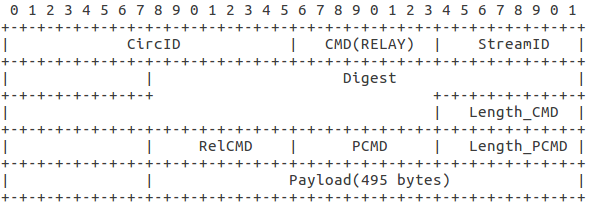
\includegraphics[scale=0.38]{images/payment_cell_header.png}
%    \caption{Relay Payment Cell --- Cell definition specifying the structure of
%      a moneTor payment cell. Note: a block that appears blank and empty is in fact the continuity of the previous row}
%\label{fig:relay_command_mt_structure}
%\end{figure}
%
%All the bytes starting from StreamID (included) are onion encrypted. RelCMD is set to RELAY\_COMMAND\_MT, PCMD is the payment command which is different for each step of the payment protocol. If some message overflows the payload available length (495 bytes), we queue multiple cells of the same PCMD and buffer them on the receiver side to unpack the whole message.

\subsection{Pre-built Channels}
By default, Tor attempts to pre-build circuits in order to reduce latency once a
user wishes to create a data stream. Much like circuits, moneTor payment
channels are high in initial latency because of the many in-out messages in the protocol. We therefore exploit the same strategy currently used in circuit establishment by
allowing payment channels to be preemptively set up and established on clean
pre-built circuits. This dramatically reduces the effective time to first
payment. Unfortunately, excessive establishment of preemptive channels will
eventually afflict the network with unused overhead. Our implementation features
a rudimentary prediction strategy that attempts to balance this trade-off by
anticipating the number of needed channels using historical usage
information in a similar way Tor anticipates the need for a fresh circuit.
%However, our approach may not be sufficiently optimized and further
%work on this front is warranted.

\subsection{Network Scalability}
\label{subsub:scalability}
%\td{TODO: describe scalability of intermediary system and any networking
%  bottlenecks that might arise such as port limits, etc.}

In our design, we are concerned with memory consumption, kernel socket
consumption and CPU consumption. Our choice for a tripartite protocol
effectively shifts the memory consumption of opened and idle micro
channels to the intermediary nodes of the network. A more basic setup
whereby each Tor client maintains a micropayment channel with each
relay would incur an $O(n*m)$ cost with
respect to channel management complexity, with $n$ the number of Tor clients and $m$ the number of relays. By engineering an additional
intermediary layer, the complexity of moneTor channel connections is
reduced to $O(n+m)$. In our implementation, intermediary relays do not
participate in routing user streams and are tasked only with providing
payment channel services. Intermediaries devote the full extent of
their computational resources toward this task, allowing only a few
strong nodes to handle all of channel management needs of the network.

Interactions between parties are realized within Tor circuits to allow
multiplexing of circuits over the same TCP connection. This also protects the
identity of the client and its chosen circuit against identification by the
ledger or the intermediary\footnote{We assumed no side-channel exploitation in
  this work but do discuss timing attacks in
  Section~\ref{sec:limitations_futurework}}. As a result, the intermediary and
the ledger must have a number of available sockets higher than the number of
relays in the network in the worst case. Since this limit is in line with Tor's
current assumption, our design inherits the same socket consumption scalability
of the greater Tor network.

\subsection{Prioritized Traffic}
\label{subsub:prioritized}

The final component of our network-oriented design addresses the need to deliver
prioritized bandwidth given an explicit signalling of premium or nonpremium
traffic. Our objective is to provide a tunable range of prioritization while
incurring as little cost as possible to average global performance. In our
design, the chosen value is enforced network-wide by the directory authorities
in order to avoid partitioning of the anonymity set. Traffic scheduling is
perhaps the most intuitive mechanism with which to implement
prioritization. However, we found in our investigation that practical
modification of the Tor scheduling infrastructure is nontrivial. A more detailed
discussion of our findings can be found in Appendix~\ref{sec:scheduling}.

Fortunately, Tor's overlay flow control mechanism provides an alternative route
to implement our desired functionality. Recall that edge nodes regulate the
traffic flux in either direction using a set of flow control windows. Roughly
speaking, these windows determine space allotted to each circuit on a relay's
scheduling queue, which in turn is positively correlated with effective
bandwidth. We implement our prioritization scheme by readjusting the windows
according to the following formula.
\begin{equation}
  window' = window(1+ \alpha(premium / premium\% - 1))
  \label{eq:flow}
\end{equation}
Here, a circuit is marked as prioritized by the bit
$premium \in \{0, 1\}$. The tunable priority benefit
$\alpha \in [0, 1)$ defines the proportion of the non-premium capacity that we wish
to transfer to premium clients. By accounting for
$premium\%s \in [0,1]$, the fraction of premium to nonpremium clients, we
can keep the total flow capacity constant. 
%Our policy may be
%implemented in one of two ways. First, each node could track the
%$premium\%$ locally and dynamically adjust their own windows. This
%introduces a considerable amount of added complexity with unclear
%consequences on network performance. A more sound approach calls for
%the Tor authorities to track the global value for $premium\%$ and
%periodically broadcast static flow control windows to be used by the
%entire network. We adopt the latter approach in this iteration of
%moneTor.

\paragraph*{Interlude.} This concludes the design of the moneTor framework. In
the proceeding sections, we describe steps taken to iteratively select and
validate key parameters as well as the scheme as a whole. Such parameters
include: payment frequency, preemptive channel creation, and prioritization
amounts ($\alpha$). Throughout this process, the underlying objective is to
prove that we can confer qualitatively ``significant'' advantage to paid premium
users while incurring minimal overhead costs with respect to throughput, memory
usage, and latency within a realistic network environment.

%\footnote{Our
%  research in traffic prioritization is meant to demonstrate at least some crude
%  capacity for premium advantage in our models and to suggest potential avenues
%  for further study. A more definitive design for production-ready policies is
%  left for future networking-oriented research.}

%%% Local Variables:
%%% mode: latex
%%% TeX-master: "../main"
%%% End:


\section{Empirical Analysis}
\label{sec:analysis}
%\op{Is it only validation? It seems that some of the paramters are also chosen based on these simulations. Also, the discussion seems to be using some parameters which are only made explicit later. For instance, in 7.1.2, the circuits with less than 1000 cells are described as useless for premium. The reson for that seems to only become clear when reading 8.3.1, which indicates that payments are made after 1000 cells. I wonder if, at the end of this section, and before the experimental analysis, it would make sense to add a frame that sums-up what protocol will be analyzed, including the parameters: what channels and circuits are created when, when is payment happening, when are channels closed, \dots}

\subsection{Data Collection}
\label{subsec:datacollection}

We deployed during two weeks a data collection system to look for empirical temporal information
about lifetime and bandwidth consumption in Tor circuits. Our objective was to
have a deeper understanding of typical Tor usage and whether such usage can
benefit from our channel-based payment system. For example, these measurements
might capture some notion about the type and magnitude of potential premium
traffic. We classify the traffic type based on the service connection
port. Besides the classical ports 80 and 443 used for web traffic, we aggregate
data from some other families including the WHOIS
protocol~\cite{daigle2004whois} and RWHOIS~\cite{williamson1994referral} from
ports 43 and 4321, respectively. The complete list of families is constructed
from the reduced exit policies which we run on our relays. This measurement
methodology allows us to reason based on application specific traffic.

% We interested to know about the distribution lifetime of Tor circuits for each
% port we allow. We are also interested to picture how many cells those circuits
% handled through their lifetime with some level of granularity.

\subsubsection{Efforts to preserve users privacy}

To ensure ethical experimentation, we first contacted the Tor research safety
board~\cite{torsafety}. The feedback we received was subsequently used to refactor our data
collection process (e.g., no metadata from any specific flow or circuit should be written on disk).

Data from five old and very stable exit relays with a total bandwidth of 50 MiB/s was collected, stripped of
origin metadata, and aggregated on a central server. The data collected from each
relay is itself an aggregation which we perform inside the relay's memory. The aggregation is done only for ``active circuits'' from the exit relay perspective. We consider a circuit active when it has received a connection request to an IP address on the internet.
%The data collection is probabilistic; only 30\% of the circuits processed by our
%relays were considered in order to maintain plausible deniability on the
%clients' behalf.
The aggregation is done inside bins of configurable size for
every different traffic family we consider. Once we collected enough data from a
single family, we dump the information on the disk, clear the data, and resume a
new session. The final information obtained contains an aggregation of 1600
circuits over an unspecified time frame that is implicitly determined by the
rate of user activity. The following data was considered:

\begin{itemize}
\item \textbf{Time Profile}: The number of cells in each time interval
  (configured to be 5 seconds) since the success of the DNS request. This
  information sums inbound and outbound cells, and is aggregated over circuits
  by addition.
\item \textbf{Total Counts}: The total amount of cells processed by a
  circuit. This information is aggregated by taking the mean of fixed-size
  nearest neighbor bins.
\end{itemize}

Crucially, we do not record information linked to any single particular user
flow on disk.
%The code used for the data collection will be made available for
%audit online.

\subsubsection{Observations}

\begin{figure} \centering
  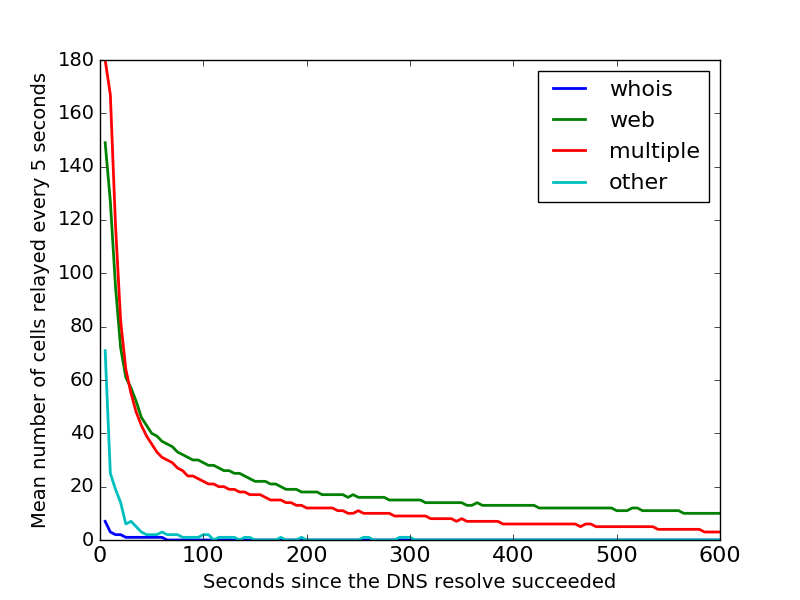
\includegraphics[width=0.4\textwidth]{images/exitmeasurement.png}
  \caption{Time Profile --- Average distribution of traffic across circuit
    lifetime beginning with the first DNS request.}
  \label{fig:statsa}
\end{figure}
\begin{figure} \centering
  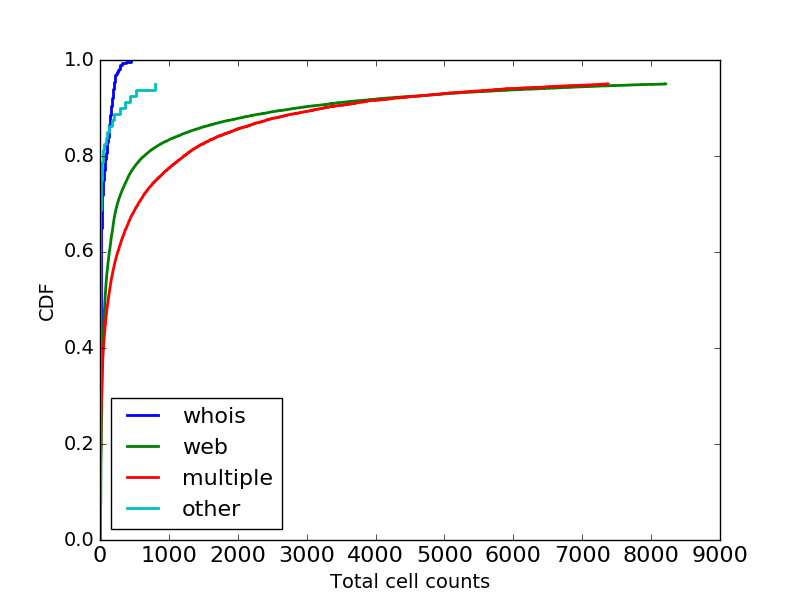
\includegraphics[width=0.4\textwidth]{images/totcellcountscdf.png}
  \caption{Total Counts --- Distribution of circuit size with respect to the
    total number of cells processed}
\label{fig:statsb}
\end{figure}


Our measurements successfully captured several important pieces of information
for the design and justification of moneTor. For example, one important task is
to determine the number of potential users that could benefit from paid
traffic. From Figure~\ref{fig:statsb}, we observe that $\approx 82\%$ of
circuits carrying only web traffic exchanged less than 1000 cells. While we
cannot deduce any statements about users, we can speak to the fraction of
circuits that may benefit from a payment channel in the Tor network, since
around $50\%$ of them do not carry data and less than $17\%$ of them carry at
least one web page. The remaining $18\%$ would appear to be better candidates
for moneTor.

It is also evident from Figure~\ref{fig:statsa} that most of the traffic is usually
carried within the first few tens of seconds, and that all types of traffic we
collected seems to follow the same rule. From that result, we believe that the
reliability of payment is critical within the first few seconds, especially from
a relay viewpoint. Our payment channels should ideally be established and ready
before the user begins to use the circuit. While this result cannot be
guaranteed for an unbounded number of circuits, a well-designed preemptive
circuit build strategy should do a sufficient job of eliminating channel
setup/establish latency in the average case.

%% In another area of research, it may be interesting to point out that since %
%$\approx 50\%$ of users do not carry data after their DNS request, some %
%adversary doing end-to-end correlation may prefer to use active attacks over %
%passive correlation to capture more identities.

\section{Simulated Validation}
\label{sec:experimentations}

Having established the empirical context for a channel payment scheme, we
validated our technical design via experiments performed on a prototype
software implementation within the native Tor codebase.

\subsection{Prototype}

A substantial contribution of the research is embedded within our implementation
of the moneTor framework. The modifications, applied to Tor release version
0.3.2.10, cover approximately fifteen thousand added lines of code across Tor's
core C software. We emphasize that the implementation is not a fully functional
prototype and is optimized solely for our experiments. Most notably, we
simulated crytographic operations in the nanopayment creation and close
procedures using CPU delays. These delays were tuned to conservatively reflect
real measurements in background work~\cite{green2017bolt}.\footnote{Extracted
  values are conservative in the sense that our zero-knowledge proofs require
  proving only a subset of the statements required in each corresponding Bolt
  zero-knowledge proof.} The partial prototype serves the following purposes in
our study.

\begin{enumerate}
\item An implementation covering nuances not explicitly
  covered in the protocol designs. In effect, we would like to show that there
  are no unexpected and prohibitive practical conflicts with the existing Tor
  design.
\item A platform to study the feasibility of premium circuit
  prioritization from a networking perspective.
\item A platform to obtain a rough factor-of-two approximation for all
  bandwidth, computation, and memory requirements of the system, both globally
  and at individual nodes.
\end{enumerate}

The first design purpose is clearly qualitative and we briefly note that we did
not discover any insurmountable logical flaws in the design. To analyze the
networking dynamics and resource consumption, we studied our implementations
through the following proceeding experiments.

\subsection{Methodology}
\label{subsec:methodology}

Experiments were conducted using the Tor shadow simulator
tool~\cite{jansen2011shadow}. We ran two sets of experiments at different
scales from a consensus document published in early February 2018. The first set featured 100 relays, 1000 clients, 10 intermediaries, and
ran for a total of 90 minutes. These experiments were used to gather information
concerning the system overhead and protocol execution times. The second set
featured 250 relays, 2500 clients, 25 intermediaries, 80 minutes of total run
time, and was used to measure the performance benefits conferred to premium
clients. In both cases, simulated traffic features 16\% \emph{bulk} clients who
continuously download 5 MiB files and 84\% \emph{web} clients who periodically
download 2 MiB files,\footnote{While 5 MiB bulk files are a common standard in
  Tor benchmarking~\cite{portal2018tormetrics}, 2 MiB web files reflect the
  approximate size of modern web pages~\cite{team2018httparchive}}. The number
and behavior of clients were chosen to satisfy (A) realistic congestion rates
measured by a transfer timeout percentage around 4\%~\cite{portal2018tormetrics}
and a historical bulk/web global traffic ratio of about
50\%~\cite{chaabane2010digging, mccoy2008shining}. Importantly, it should be
noted that neither the scale of our experiments nor the precise configuration of
client nodes are intended to be precise replicas of real-world conditions. Tor
networking is itself a complex area of research and we are content to adopt the
simplest model that will highlight the relatively crude networking needs of our
incentivization scheme.

\subsection{Experiments}
\label{subsec:experiments}
Our experiments are separated into three groups each capturing a separate
characteristic of the scheme.

\subsubsection{Global Overhead}

First, we attempt to show the total cost the moneTor scheme in terms of total
network throughput. To highlight worst-case performance, we configured a medium
scale experiment consisting of 100\% of premium clients and compare to a
baseline trial with 0\% premium clients. No actual traffic priority is
conferred. Since our algorithms makes use of some concurrent crytpographic
operations, we are concerned with the number of CPU cores available to most
relays. This information is not publicly available. As a result, we 
provide two trials with moneTor: one where we assume all nodes are running on
multi-core hardware and one in which all nodes are running on single-core
hardware. The results are summarized in Figure~\ref{fig:overhead}.

% Add information about how we simulate singlecore and multicore hardware
% That gonna overflow 12 pages, though :/

\begin{figure*} \centering
	\begin{subfigure}[t]{0.32\textwidth} \centering
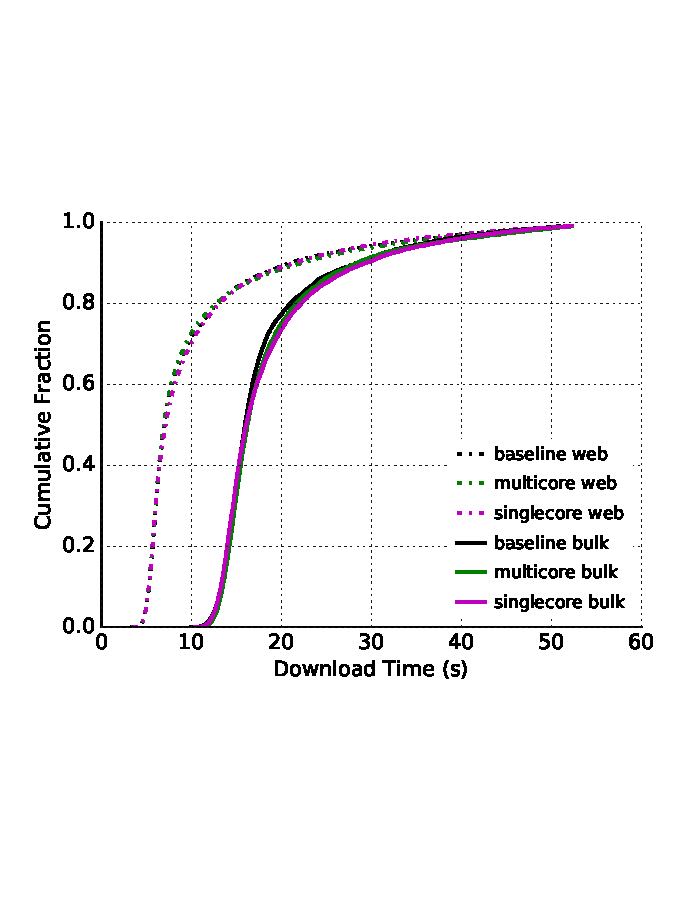
\includegraphics[trim={0 3cm 0 3cm}, clip, width=1.0\textwidth]{images/overhead_downloadtime.pdf}
		\caption{Download Time Overhead}
		\label{fig:overhead_ttlastbyte}
	\end{subfigure}
	\begin{subfigure}[t]{0.32\textwidth} \centering
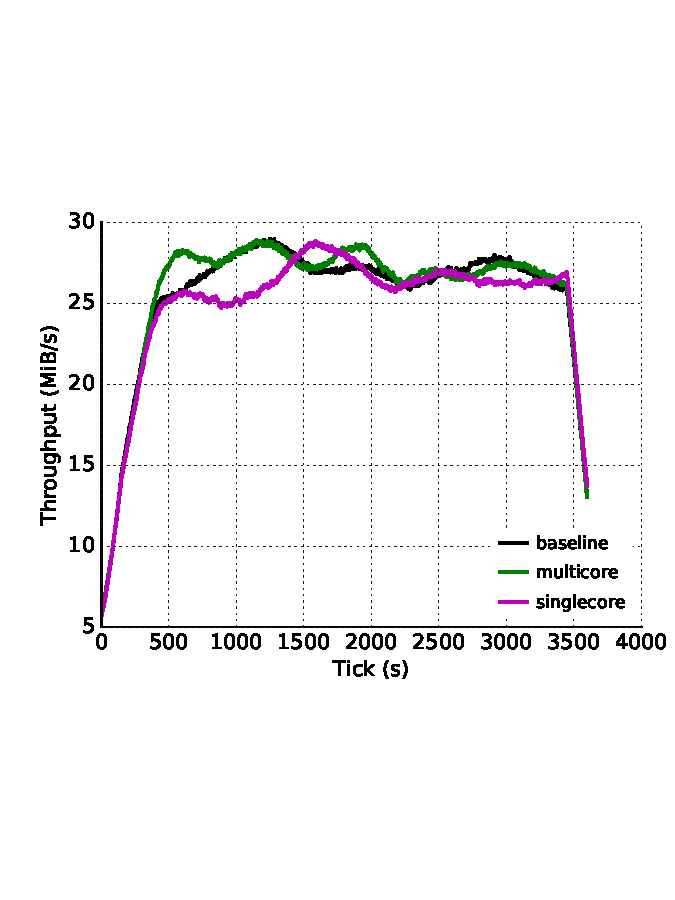
\includegraphics[trim={0 3cm 0 3cm}, clip, width=1.0\textwidth]{images/overhead_throughput.pdf}
		\caption{Throughput Overhead}
		\label{fig:overhead_throughput}
	\end{subfigure}
	\begin{subfigure}[t]{0.32\textwidth} \centering
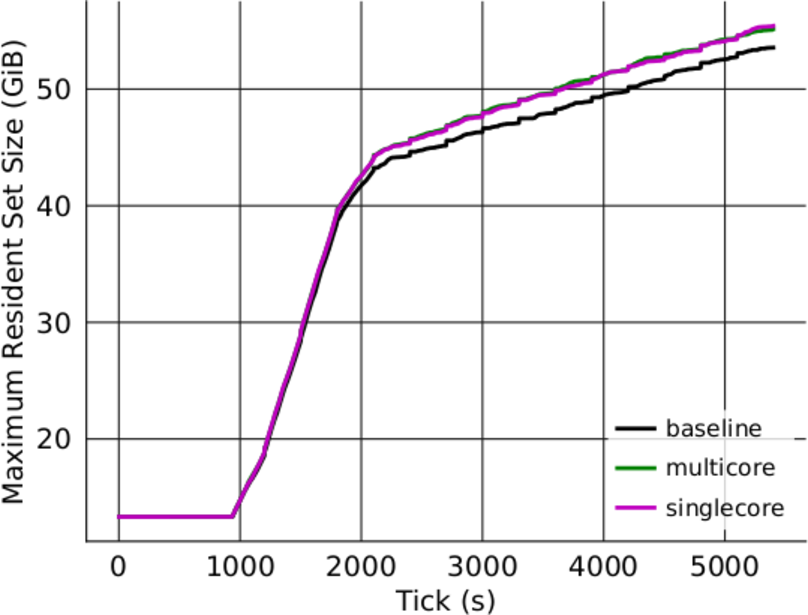
\includegraphics[trim={0 3cm 0 3cm}, clip, width=1.0\textwidth]{images/overhead_memory.pdf}
		\caption{Simulation Memory}
		\label{fig:overhead_shadow}
	\end{subfigure}
	\caption{Global Overhead --- Comparison of overhead in pure multicore
          and singlecore network
          conditions. Figure~\ref{fig:overhead_ttlastbyte} shows two sets of
          download time CDF curves for each file size (2 MiB and 5 MiB),
          Figure~\ref{fig:overhead_throughput} shoes the 5 minute moving average
          throughput over time, and Figure~\ref{fig:overhead_shadow} shows the
          memory consumption across the experiment lifetime. The simulation
          includes 100 relays, 2 authorities, 1 ledger authority, 10
          intermediaries and 1000 Tor clients scaled down from the public
          consensus file `2018-02-03-00-00-00-consensus'.}
	\label{fig:overhead}
\end{figure*}

Our findings indicate that even in the worst case scenario, our system incurs
statistically negligible overhead at these scales across all three measures of
download time, throughput, and memory usage. This in line with the raw bandwidth
overhead observations in which a small fraction ($< 1\%$) of the network traffic
is attributable to moneTor payment messages. This is true for all of our trials
which feature a payment rate of 1 payment (1 cell) every 1000 data cells
exchanged in either direction. It is also possible to increase the payment rate
for more fairness if needed, as long as the total overhead induced from control
cells is kept under an acceptable fraction of the overall data bandwidth. 
%%%
% Reading this sentence appears to be unclear to me
%%%
%This
%low overhead cost is separate from adverse networking effects of prioritization,
%which has the potential to more drastically affect performance.

%\begin{table}
%  \caption[Overhead Throughput Total]{\textbf{Overhead Throughput Total} Total
%    transferred application traffic over the duration of the over head trials
%    compared to total transferred payment traffic.}
%  \begin{center}
%    \begin{tabular}{ c c c }
%      & Throughput (GiB) & Payment Traffic (GiB) \\ \hline
%      Baseline & 128.4 & 0.000 \\
%      Multi-Core & 129.1 & 0.449 \\
%      Single-Core & 127.6 & 0.396
%    \end{tabular}
%  \end{center}
%  \label{tab:overhead}
%\end{table}

\subsubsection{Payment Latency}

Given results from our data collection, we surmise that payment latency is a
crucial factor in servicing our front-loaded clients. To this end, we measure
the distribution of completion times for various steps in the protocol. The
results shown here are collected from a worst case multicore experiment
featuring 100 relays and 1000 clients all of whom run premium circuits. To
highlight the effects of native latency in the Tor network, we show payments
split across each relay role of guard, middle, and exit. Recall that moneTor
makes use of high-overhead, low-marginal cost payment channels. The bulk of the
cost in our scheme lies in the conduction of the nanopayment channel
\emph{establish} and \emph{close} protocols as shown in
Figure~\ref{fig:payments_establish} and Figure~\ref{fig:payments_close}. Notice
that close operations are about twice as time consuming as establish operations
reflecting the need for the relay to close his half of the nanopayment channel
before the client can complete hers. Figure~\ref{fig:ttfp} illustrates time to
first payment, our most revealing latency metric. This measure includes the
overhead in channel establishment when we do not have available preemptive
channels. In the best case scenario, when all three payment channels have been
correctly pre-built for the circuit, this measure is equivalent to a single trip
toward each relay. Comparing this Figure~\ref{fig:ttfp} to
Figure~\ref{fig:payments_establish}, we observe the effectiveness of preemptive
channel building.

\begin{figure*} \centering
	\begin{subfigure}[t]{0.32\textwidth} \centering
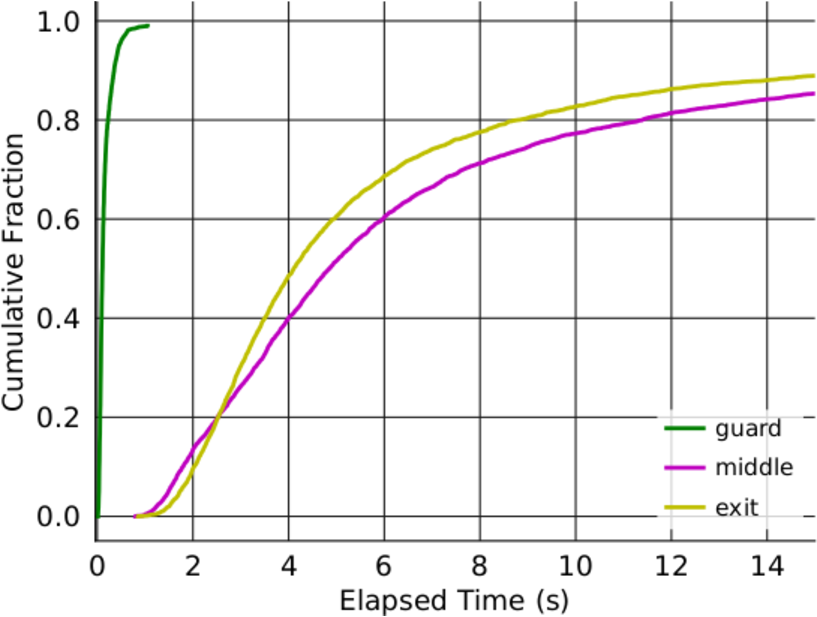
\includegraphics[trim={0 3cm 0 3cm}, clip, width=1.0\textwidth]{images/payment_establish.pdf}
		\caption{Nano-Establish}
\label{fig:payments_establish}
	\end{subfigure}
	\begin{subfigure}[t]{0.32\textwidth} \centering
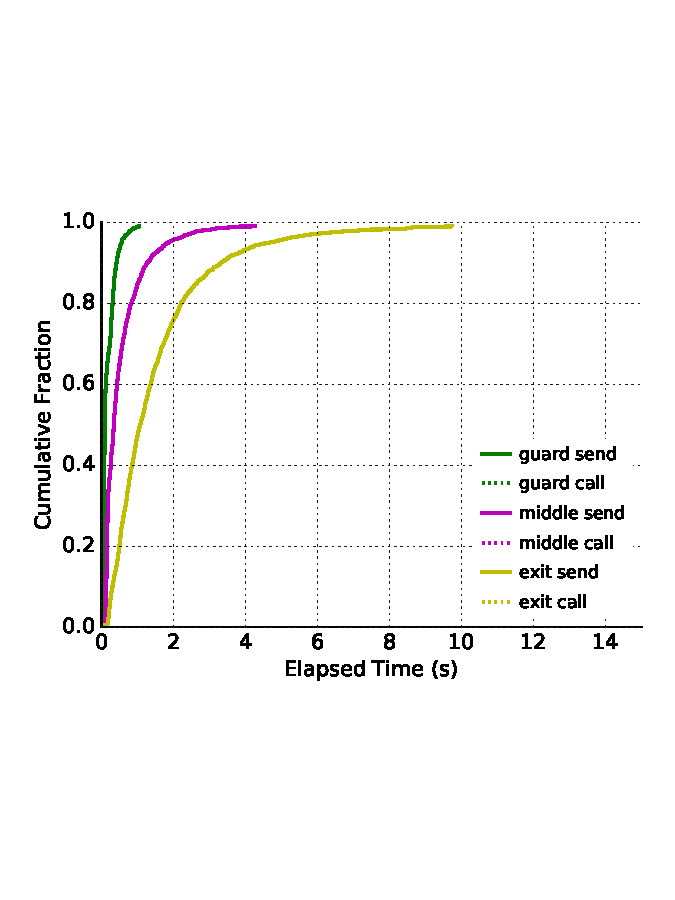
\includegraphics[trim={0 3cm 0 3cm}, clip, width=1.0\textwidth]{images/payment_pay.pdf}
		\caption{First Payment}
\label{fig:ttfp}
	\end{subfigure}
	\begin{subfigure}[t]{0.32\textwidth} \centering
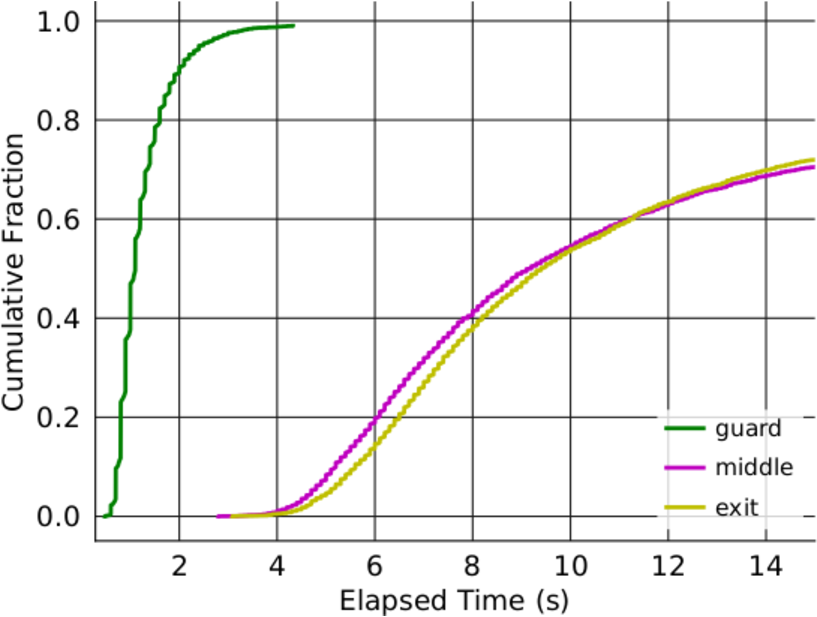
\includegraphics[trim={0 3cm 0 3cm}, clip, width=1.0\textwidth]{images/payment_close.pdf}
		\caption{Nano-Close}
\label{fig:payments_close}
	\end{subfigure}
	\caption{Protocol Execution Time --- Time to finish each protocol step
          split across interactions with each of the three relay. The simulation
          includes 100 relays, 2 authorities, 1 ledger authority, 10
          intermediaries and 1000 Tor clients scaled down from the public
          consensus file `2018-02-03-00-00-00-consensus'.}
\label{fig:latencymeasurements}
\end{figure*}

In all protocol phases, we observe that latency for guard relays are negligible
in comparison to the middle and exit relays, further validating our design
decision to implement special directly paid guard channels.

\subsubsection{Network Priority}
\label{sec:priority_exp}

Our final set of experiments studies the success of our scheme in delivering
prioritized traffic for premium users. To perform this analysis, we prepared
sets of three small experiments with varying modifier priorities
$\alpha \in \{0, 0.25, 0.5\}$, where $\alpha = 0$ represents the baseline
control. Our first set of experiments assuming 50\% of premium users is shown in
Figures \ref{fig:modifier_pr50_web}, \ref{fig:modifier_pr50_bulk}, and
\ref{fig:modifier_pr50_all}. From this illustration, is it evident that premium
users enjoy an advantage in internet speed compared to nonpremium users and that
this advantage is more pronounced with the higher priority modifier. Moreover,
the evenly split premium and nonpremium performance ``averages out'' to
approximately mirror the baseline experiment, indicating little loss in overall
network performance, and confirming our overhead experiment.

A more realistic model should most likely assume a smaller minority of premium
users. We therefore conducted a separate set of experiments to study an
environment comprised of only 25\% premium users who, according to
Equation~\ref{eq:flow}, should expect an even greater benefit on a per-user
basis. Figures \ref{fig:modifier_pr25_web}, \ref{fig:modifier_pr25_bulk}, and
\ref{fig:modifier_pr25_all} shows that this is indeed the result. Users across
the spectrum of web speed enjoyed $\approx 100\%$ improvements in download
speeds relative to nonpremium users --- likely enough to induce some amount of
monetary exchange. 


\begin{figure*} \centering
	\begin{subfigure}[t]{0.32\textwidth} \centering
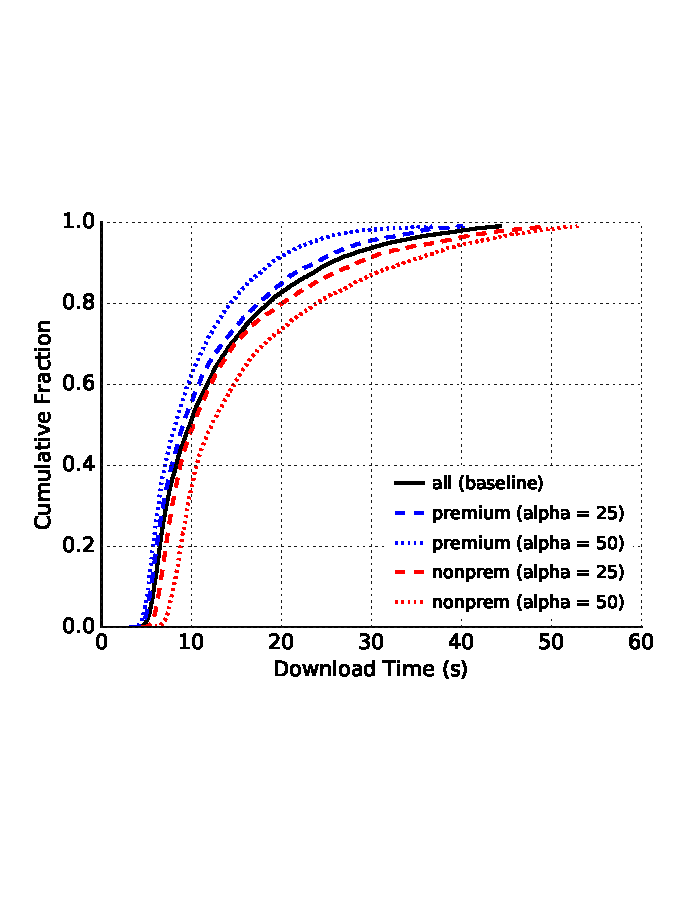
\includegraphics[trim={0 3cm 0 3cm}, clip, width=1.0\textwidth]{images/modifier_pr50_web.pdf}
		\caption{Web Download Time}
\label{fig:modifier_pr50_web}
	\end{subfigure}
	\begin{subfigure}[t]{0.32\textwidth} \centering
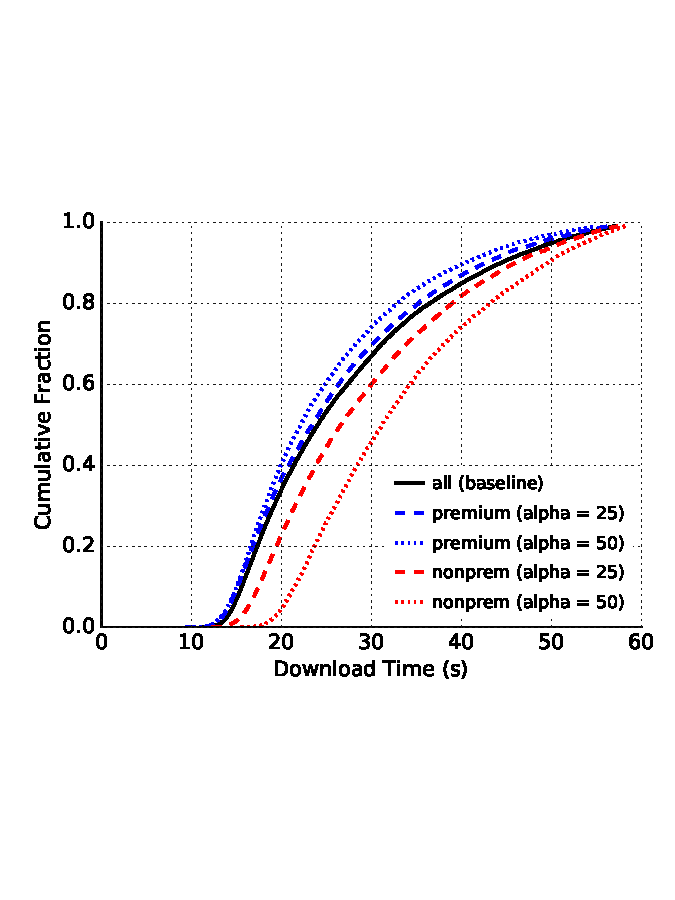
\includegraphics[trim={0 3cm 0 3cm}, clip, width=1.0\textwidth]{images/modifier_pr50_bulk.pdf}
		\caption{Bulk Download Time}
\label{fig:modifier_pr50_bulk}
	\end{subfigure}
	\begin{subfigure}[t]{0.32\textwidth} \centering
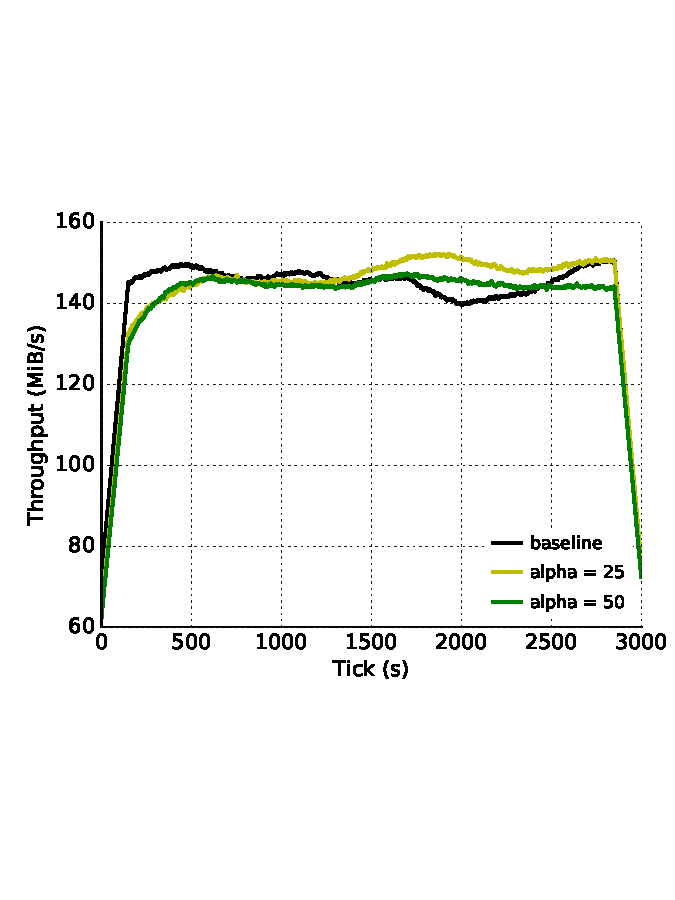
\includegraphics[trim={0 3cm 0 3cm}, clip, width=1.0\textwidth]{images/modifier_pr50_all.pdf}
		\caption{Throughput}
\label{fig:modifier_pr50_all}
	\end{subfigure}
	\begin{subfigure}[t]{0.32\textwidth} \centering
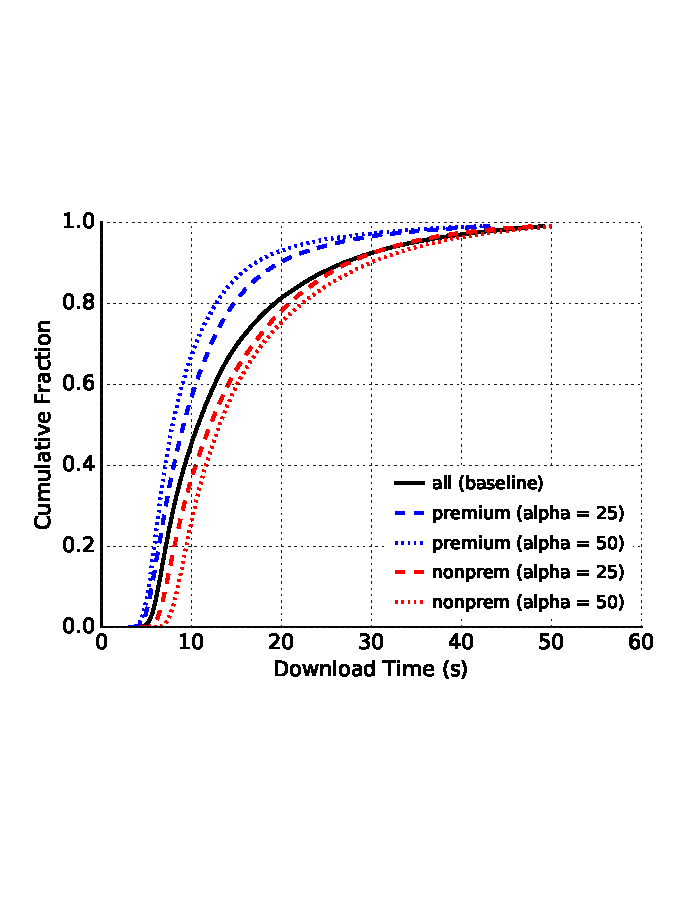
\includegraphics[trim={0 3cm 0 3cm}, clip, width=1.0\textwidth]{images/modifier_pr25_web.pdf}
		\caption{Web Download Time}
\label{fig:modifier_pr25_web}
	\end{subfigure}
	\begin{subfigure}[t]{0.32\textwidth} \centering
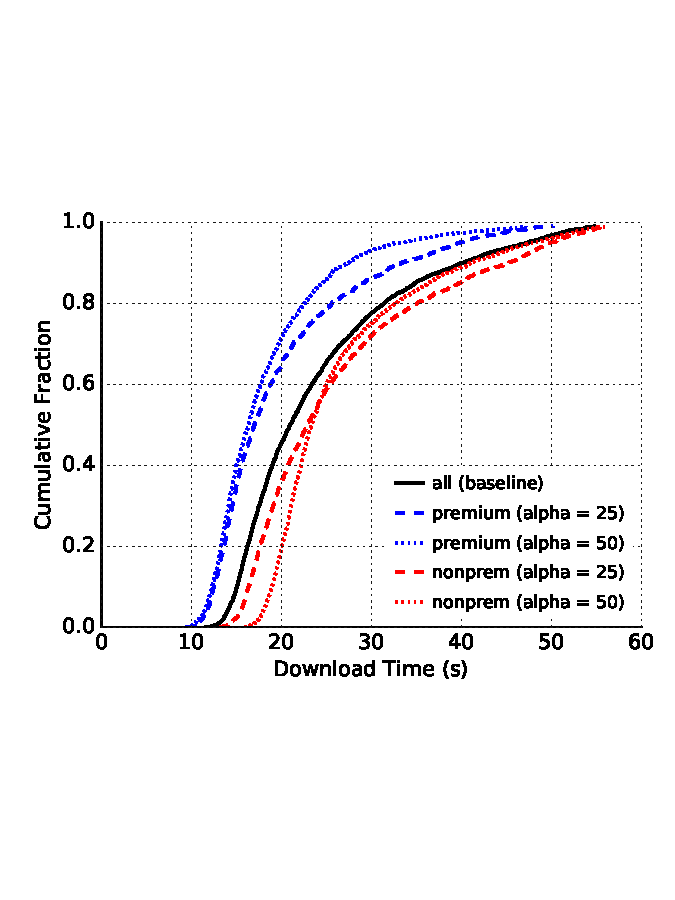
\includegraphics[trim={0 3cm 0 3cm}, clip, width=1.0\textwidth]{images/modifier_pr25_bulk.pdf}
		\caption{Bulk Download Time}
\label{fig:modifier_pr25_bulk}
	\end{subfigure}
	\begin{subfigure}[t]{0.32\textwidth} \centering
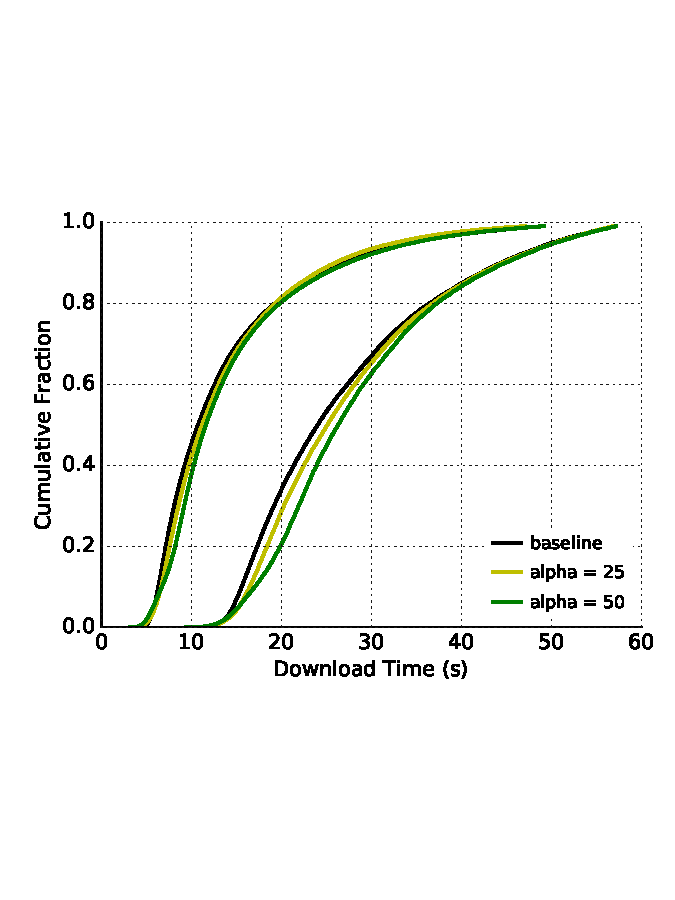
\includegraphics[trim={0 3cm 0 3cm}, clip, width=1.0\textwidth]{images/modifier_pr25_all.pdf}
		\caption{Throughput}
\label{fig:modifier_pr25_all}
	\end{subfigure}
	\caption{Prioritization Benefit --- Performance differentiation between
          paid and unpaid users. The first row displays results with 50\%
          premium users while the second row displays results for 25\% premium
          users. Simulations feature 250 relays, 2 authorities, 1 ledger
          authority, 25 intermediaries and 2500 Tor clients scaled down from the
          public consensus file `2018-02-03-00-00-00-consensus'.}
\label{fig:modifier}
\end{figure*}

%\begin{table}
%  \caption[Prioritized Throughput]{\textbf{Prioritized Throughput} Tabulate total
%    number of successful file transfers and timeout errors across varying levels
%    of prioritization}
%  \begin{center}
%    \begin{tabular}{ c c c c}
%      & Throughput & Timeouts & Timeout \\
%      & (GiB) & (Web) & (Bulk) \\ \hline
%      $\alpha = 0.00$ & 427 & 115 & 354 \\ \hline
%      $\alpha = 0.25,\ pr\% = 50$ & 429 & 206 & 404 \\
%      $\alpha = 0.25,\ pr\% = 25$ & 433 & 231 & 459 \\ \hline
%      $\alpha = 0.50,\ pr\% = 50$ & 420 & 233 & 356 \\
%      $\alpha = 0.50,\ pr\% = 25$ & 414 & 381 & 513 \\
%    \end{tabular}
%  \end{center}
%  \label{tab:modifier}
%\end{table}

%%% Local Variables:
%%% mode: latex
%%% TeX-master: "../main"
%%% End:


\section{Related Work}
\label{sec:related_work}
We classify the previously proposed incentivization schemes into three groups:

\noindent \emph{1. Non-transferable benefits:} these proposals aim to recruit
relays by offering some privileged status intended for personal use which cannot
be \emph{securely} sold for reimbursement of financial
investment~\cite{dingledine2010building,jansen2010recruiting, jansen2013lira}.
Current state-of-the art schemes for Tor incentives are in this category and the
next one, and we focus our comparison to them.
	  
\noindent \emph{2. Transferable benefits:} these schemes offer privileges or
products intended to hold value in a secondary resale market. These indirect
financial incentives presume to attract a broader demand than in the
non-transferable case. Partial proof-of-work tokens that can then be redeemed by
relays for profit in real cryptocurrency mining pools~\cite{biryukov2015proof}
and exchangeable shallots in TEARS~\cite{jansen2014onions} are part of this
category.

\noindent \emph{3. Monetary payments:} these schemes offer rewards with what
might be considered real money that holds external value.
PAR~\cite{androulaki2008payment} allows clients to send direct payments to
relays in a hybrid payment scheme which makes use of inefficient but anonymous
Chaumian e-cash protocols~\cite{chaum1988untraceable} and efficient but
transparent probabilistic micropayments. PAR introduces the \emph{honest but
  curious} bank paradigm in which the bank cannot deanonymize clients but is in
control of their deposited financial assets. PAR suffers from scalability issues
owing to its strongly centralized architecture. Other monetary payments schemes
such as Xpay~\cite{chen2009xpay} and the proposal of Carbunar~\textit{et
  al.}~\cite{carbunar2012tipping} are limited by the same \emph{honest but
  curious} security assumptions and their scalability remains capped by the need
for all clients to interact with the central bank for each payment chain. The
moneTor scheme can be seen as a member of this family of solutions, with the
following advances: moneTor removes the need to rely on a \textit{honest but
  curious} bank, and offers a solution to the scalability issue inherent to
previous approaches.


%\footnote{Generally speaking, incentives provided by monetary payments
%  are more economically robust than transferable benefits, which in turn are
%  more robust than non-transferable benefits. Although we examine related works
%  through the prism of economic appeal, this is not a statement of superiority
%  so much as an observation on diverging motivation. Indeed, a number of
%  sociological and legal implications must be weighed before
%  introducing financial profitability into the Tor ecosystem. We consider these
%  to be out of scope for the purposes of our research.}

%\op{Need to explain why our solution is better/more interesting than all these.}

%\paragraph*{Non-transferable benefits - Gold Star} As one of the earliest
%incentive proposals, Gold Star introduces the notion of premium bandwidth.
%Premium, or \emph{gold star} status, is awarded exclusively to the fastest 7/8
%fraction of relays, signalling to the rest of the network that these relays can
%enjoy prioritized traffic. While highly attractive for its conceptual
%simplicity, Gold Star leaks a considerable amount of user information since
%priortized traffic can now be trivially attributed to this relatively small set
%of gold star relays~\cite{dingledine2010building}, since gold star is by design
%non-transferable.

We now review these approaches in more details.

\paragraph*{Non-transferable benefits - BRAIDS/LIRA} The BRAIDS scheme
introduces \emph{tickets} to represent premium status. Users may wish to
transfer tickets to other users, but this transfer must be done through a
trusted-third party. Small numbers of ephemeral tickets are freely distributed
by a central \emph{bank} to any client upon request or to relays that have
accumulated tickets spent by clients. Crucially, tickets can only be spent at a
single relay defined at the time of their minting, in order to circumvent the
double spending problem~\cite{jansen2010recruiting}, yet those tickets can be
exchanged at the bank for others bound to a new relay assuming that the exchange
happens within the allowed time interval. BRAIDS raises four major concerns:
1)~everyone connects to a central bank through Tor, which raises scalability
issues; 2) the bank is not trustless: by design the bank can issue valid tickets
for anyone, and guard relays can steal tickets in the distribution process; 3)
verifying a blind signature on relay side for each payment is computationally
intensive if the rate of payment is high, and current high-bandwidth Tor relays
are already CPU-bound; 4) interactions with the bank is increased by the fact
that tickets are designed to be relay-specific. As a consequence, BRAIDS can
hardly scale as a result of an economic appeal: as the size of the network
increases, users must either stockpile an increasing number of tickets for all
the relays they may use or need to interact more and more frequently with the
bank to exchange them.

LIRA is an ideological successor to BRAIDS which reduces scalability issues and
improves the efficiency of the relay side verification of tickets by a factor
$\approx 80$. Clients in LIRA probabilistically ``win'' premium tickets without
any interaction with the bank. While LIRA improves the efficiency of BRAIDS, and
could even offer high fairness (by supporting high payment rates), it suffers
from a \textit{client} cheating incentive to continuously build circuits to try
to win premium tickets~\cite{jansen2013lira, jansenblogpost}. Depending on the
chosen value for the payment rate, this problem by itself could prevent the
scheme from offering a realistic option. If the payment rate is too low, then
the incentive to cheat is increased because a large priority bandwidth would be
rewarded between guesses to the cheater. If a high payment rate is chosen, then
guessers would have difficulties to maintain good guesses through their circuit
lifetime (as the probability to maintain priority through guesses exponentially
decreases). As a result, the LIRA idea to have increasing buyer anonymity
through successful guessers is losing its efficacy. Moreover, LIRA does not
address Concerns 2) and 4) inherited from BRAIDS.

Compared to BRAIDS and LIRA, moneTor offers the ability to prevent
double-spending without suffering from a centralized exchange process
(BRAIDS)~\cite{jansenblogpost}, or from incentives to cheat to gain premium
access and stockpile relay-specific information (LIRA). Moreover, moneTor offers
high fairness with on-the-fly payment verification improved by a factor $\approx
6$ compared to LIRA (one $\hash$ operation instead of six $\hash$ + a few XORs
and multiplications) and $\approx 500$ to BRAIDS. This does not account for
opening and closing the nanopayment channel, happening outside of the data
transfer time window and for which the relay's costly operation is to perform
one ZKP (opening) and generating one blind signature (closing). Also, moneTor
does not suffer from concern 2) and moneTor tokens can act as a wrapper from an
external cryptocurrency such as Bitcoin or Ethereum using inter-ledger
protocols~\cite{back2014enabling, poon2017plasma}.
%  \op{Do you mean that we need to be stuck to an
%  existing crypto-currency if we want problem 2) to be solved? I do
%  not see why, and this looks bad -- many people are likely to not
%  want to be linked to an external currency.} 
  Finally and more important, moneTor tokens are not relay-specific, which
  solves the scalability problem on the economic appeal (i.e., in moneTor,
  frozen funds are independent of the network size).
%Finally, moneTor payments offer to the relays what we could consider real
%money, that can be transferred or used to buy premium bandwidth directly (while
%in LIRA and BRAIDS, an exchange process with the bank is needed).

\paragraph*{Transferable benefits - TEARS} TEARS introduces a two-layer approach
whereby \emph{shallots} token are awarded by a distributed semi-trusted bank to
participating relays. These shallots, which are securely exchanged tokens, can
then be redeemed for BRAIDS-style \emph{Priority Passes}. While fully
exchangeable shallots represent an economic improvement over non-transferable
privileges, these tokens are conceptually discrete and indivisible assets that
are not as easily exchanged as true currency. We expect our ecosystem to be more
user friendly, offering arbitrarily high transferability and divisibility of
priority tokens without changing the underlying Tor architecture, while also
scaling on trustless entities (our intermediaries) instead of a distribution of
semi-trusted banks that must be operated by trusted people. The moneTor scheme
is also designed for fair-exchange with Bolt's ZKP construction to open and
close the nanopayment channels but offering $n$ nanopayments for which the relay
only has to perform $1$ $\hash$ operation to validate. This is a strong contrast
to TEARS requiring a blind signature for each payment. We also expect the
fair-exchange property to be of critical importance to enable short-bandwidth
and short-lived premium Tor circuits, which were the majority among observed
active circuits of our measurement study. Finally, a major difference with
previous work (TEARS, LIRA, BRAIDS) is that moneTor does not require to audit
relay's bandwidth to distribute tokens. Relays receive currency directly from
client from the rate of provided bandwidth and potentially more from the Tor
authorities after tax redistribution. The tax redistribution mechanism may
involve bandwidth audits, yet this is not mandatory. The counterpart of
moneTor's direct payments to the relays is that it offers an opportunity for the
exit relay to inject junk traffic (e.g., padding cells) or to conspire with the
destination to inject useless data in order to receive more nanopayments. Note
that a monitoring system to check for junk traffic could be part of the already
existing measurement system, by running premium and non-premium circuits through
measured relays. Junk traffic produced solely by the exit node is already a
severe issue~\cite{rochet2018dropping}, and the Tor project produced several
patches to observe bogus traffic and react to it. The conspirator problem is
however intractable by nature since the junk data would appear legit to the Tor
circuit layer, however our channel establishment procedure offers up to $n$
nanopayments which can be tuned to account for this problem. A conspirator can
then be reduced to non-fair exchange problem, which is what previous works offer
as a basis. Moreover, websites might not be incentivized to coerce and insert
junk traffic, given the impact it could produce on the website rendering, and to
its reactivity to user events.



%Furthermore, its reliance on a centralized bank and bandwidth
%measurement authority place implicit limits on its scalability and
%security~\cite{jansen2010recruiting}.

%\paragraph*{TorPath to TorCoin} TorCoin proposes to revamp the Tor
%architecture into one which can serve as the basis for a new cryptocurrency
%mined via a method called proof-of-bandwidth. The networking component specifies
%verifiable pseudorandom shuffling as the new method for user circuit
%selection. This modified protocol would in theory provide a weakly secure means
%for relays to mint new TorCoin tokens based on their bandwidth
%contribution~\cite{ghosh2014torpath}. Although the research is an ambitious
%attempt to simultaneously tackle many challenges including both the bandwidth
%measurement and relay incentivization problems, the authors are clear in stating
%that many questions remain regarding the security and feasibility of the scheme,
%which would in effect require a network-wide overhaul of the design of Tor.
%%While researching on TorCoin-like approach has the potential to help the Tor
%%project on one of the fundamental security problems (i.e., the bandwidth
%%measurement system), outcomes are not clear as many vulnerabilities and
%%deployment questions remain.

%\paragraph*{Transferable benefits - Proof-of-work as anonymous micropayment} Users in this simple design
%provide partial proof-of-work tokens that can then be redeemed by relays for
%profit in real cryptocurrency mining pools. The drawback of this scheme is
%simply an issue of unrealistic magnitude; the paper estimates that a user who
%continuously mines with typical consumer CPU hardware will be able to make only
%a few cents worth of payments every 24 hours while incurring a much higher cost
%in electricity~\cite{biryukov2015proof}.

%\paragraph*{Monetary Payment - PAR} A pre-Bitcoin design, PAR~\cite{androulaki2008payment}
%allows clients to send direct payments to relays in a hybrid payment scheme
%which makes use of inefficient but anonymous Chaumian e-cash
%protocols~\cite{chaum1988untraceable} and efficient but transparent
%probabilistic micropayments. PAR introduces the \emph{honest but curious} bank
%paradigm in which the bank cannot deanonymize clients but is in control of their
%deposited financial assets. As with BRAIDS, PAR suffers from an unscalable
%design owing to its centralized architecture.
%
%\paragraph*{Monetary Payment - ORPay, PlusPay, CoinPay} These three protocols, part of the
%Chaumian e-cash tradition of payments schemes, are a series of incremental
%improvements released across Xpay~\cite{chen2009xpay} and Carbunar~\textit{et al.}~\cite{carbunar2012tipping}.
% In each of the designs, the micropayment building block
%is derived from Payword hash chains~\cite{rivest1996payword}, as is ours. While
%the schemes offer practical advantages to many aspects of PAR, they are limited
%by the same \emph{honest but curious} security assumptions and their scalability
%remains capped by the need for all clients to interact with the central bank for
%each payment chain. The moneTor scheme can be seen as an idealogical member of
%this family of solutions. In the remainder of the paper, we will explain how our
%payment channel approach resolves the scalability problems inherent in the
%existing protocols and explore the auxillary implications in greater detail than
%in prior works.

%\subsubsection{Orchid} Orchid is an alternative project to Tor altogether which we
%include for thoroughness and some broad ideological similarities
%~\cite{salamon2018orchid}. It is an Ethereum-based project proposing to
%construct a brand new decentralized and market-based anonymous routing
%network. However, its stated intent focuses on censorship resistance rather
%than strong anonymity and therefore lacks comparable privacy guarantees with
%Tor. Indeed, the external payment protocol adopted by Orchid makes no claims on
%anonymity whatsoever~\cite{pass2015micropayments}.


%%% Local Variables:
%%% mode: latex
%%% TeX-master: "../popets_monetor"
%%% End:


%\section{Limitations and Future Work}
%\label{sec:limitations_futurework}
%%While we cover as much ground as possible, it has been evident from the initial
%stages that a production-ready construction of any monetary incentive scheme for
%Tor would be a monumental collaborative effort. In this final chapter, we
%discuss the promise and limitations of our results and speculate on the many
%interesting research avenues going forward.

%\subsection{Evaluation}
%\label{subsec:evaluation}
%Recall from Chapter~\ref{chap:Intro} that we are broadly concerned with three
%constraints: anonymity, economic security, and efficiency. As described in
%Chapter~\ref{chap:payment} and Chapter~\ref{chap:network}, moneTor was
%deliberately constructed to account for anonymity and economic security. We did
%not uncover any notable design flaws relating to these constraints during our
%extensive implementation phase.
%
%The results from Chapter~\ref{chap:simulation} indicate that moneTor performs
%overwhelmingly well in all efficiency measurements. This true for both global
%throughput and effective user latency where moneTor appears to achieve
%near-optimal performance in both measures. Unfortunately, we cannot produce
%meaningful comparisons with related works dealing in monetary Tor payments, as
%in all other case the researchers choose to analyze their respective algorithms
%in isolation rather than as part of a simulated Tor network. Meanwhile,
%performance comparisons with non-transferable benefit schemes and transferable
%benefits are not necessarily meaningful either, as they employ vastly different
%tokens models and should be evaluated in context. We nevertheless note that our
%decision to coordinate payments through third-party intermediaries implies that
%moneTor is conceptually more scalable than most previous proposals. A
%back-of-the-envelope calculation shows that moneTor can theoretically
%accommodate on the order of 10 million paying clients, if
%necessary.\footnote{This simple analysis conservatively assumes that the moneTor
%  ledger can handle 200 channel initiations per second (one order of magnitude
%  greater than inefficient decentralized cryptocurrencies), users are willing to
%  escrow one month's worth of payments, and users need no more than 10 concurrent
%  channels at any given time}. We are careful to acknowledge that scales
%of this this magnitude may pose any number of unseen complications which we fail
%to anticipate at the theoretical level.
%
%Finally, the paper describing LIRA is, to the best of our knowledge, the most
%recent related work that explores similar concepts of traffic prioritization in
%Tor. While it is difficult to make definitive claims comparing different
%networking simulations, we observe that our flow-control method achieves similar
%levels of traffic differentiation for the median user at lower traffic
%load~\cite{jansen2013lira}.

\subsection{Limitations}
\label{subsec:limitations}

The moneTor framework faces a number of technical and economic
limitations. Firstly, the mere presence of paid traffic leaks at least a single
bit of information to relays and intermediaries regarding the browsing habit of
the user. In practice, we expect that this information might be positively
correlated with certain user applications such as bittorrent or video
streaming. Secondly, our nanopayment protocols leak the number and value of
payments made to the intermediary. While this information cannot by itself be
used to identify clients or relays, we expect that it could provide useful
contextual knowledge when combined with other inputs. Finally, although we
ensure payment privacy within the Tor ecosystem, we can make no such guarantees
at the token exchange interface. Users who practice inadequate operational
security risk leaking information about the net value of payments they make in
Tor with their real-world identities. This problem may be of greater concern for
users residing in political regimes that are politically opposed to Tor.

A separate financial limitation arises from our our tripartite payment channel
architecture and the need for intermediaries to escrow large amounts of
funds. This opportunity cost of the frozen capital in terms of forgone
investments will be passed on as financial overhead to paying users in the form
of intermediary fees.

\subsection{Future Work}
\label{subsec:future_work}

\subsubsection{Prioritized Traffic} Although we were able to successfully demonstrate
clear prioritized premium traffic using flow control windows, there is
considerable room to analyze prioritization under more realistic settings. Among
the possibilities, we maintain that scheduling provides the most conceptually
elegant way to achieve our goals. In the absence of effective scheduling,
extension and further analysis of our flow-control technique provides an
alternative path forward. This future work might study methods for ensuring a
more robust response to local variations in the fraction of premium users as
well total network load.

\subsubsection{Side-channel Attacks} We assumed that our protocol construction would
not give more information to an observer than the single bit needed to
differentiate a premium user. However in practice, the protocol may leak
information through side-channels, such as the time needed to exchange cells in
order to open/close channels. An intermediary, or an exit relay may reason about
the client's location by evaluating the round-trip-times of the multi-rounds
protocol. Although often easily mitigated once discovered, these side channels
pose an interesting problem to our expanded attack surface.

\subsubsection{Channel Management} Given the dynamic activity of payment
channels that we have shown, further research might explore more sophisticated
policies to manage moneTor payment channels. Such policies would make decisions
concerning micropayment channel initial value, nanopayment channel size,
preemptive channel creation, and the selection of available channels to apply to
each new circuit. An ideal policy would be responsive to network load and
predicted user behavior. In addition to the classical optimization objectives of
computation, memory, and bandwidth, this research effectively considers a brand
new vector as it attempts to streamline the flow of money through the network.

\subsubsection{Extended Applications} Existing privacy-centric currencies are
limited in that they are only effective when used in conjunction with an
anonymizing network such as Tor~\cite{sasson2014zerocash}. Our currency scheme
more explicitly integrates the two layers and. This, combined with the featured
efficiency and scalability in particular makes moneTor an attractive option for
such applications as metered video viewing, metered video gaming, and
pay-per-page websites. The study and implementation of these applications in an
anonymous setting provides an interesting opportunity for multidisciplinary
research.


\section{Data Reproducibility}
\label{sec:code}
As we believe that the code should be available before acceptance, our code developed during this research and needed to reproduce our graphical results can be found in various repositories at @Monetor Github account~\cite{monetor-github}.

\section{Conclusion}
\label{sec:conclusion}
The Tor network suffers from concerns in both performance and diversity. In
accordance with the general law that large networks are better than small
networks, we assert that the quality of Tor along both of these vectors can be
simultaneously improved by incentivizing more relay participation, while
promoting some diversity notion. To this end, we present moneTor, a
comprehensive framework for incentivizing Tor relay participation through true
monetary payments. Our design broadly covers every major level of implementation
from general economic model to the protocol payment layer and integration into
the Tor networking architecture. Along the way, we developed novel protocols for
highly efficient and cryptographically secure nanopayment channels as well as
novel techniques in networking integration.

A small venture into empirical data collection reinforced our intuition that
existing user behavior is compatible with a light-weight payment incentive
scheme. This led to our more involved round of experimentation in which we
tested our natively integrated moneTor prototype. The results of this
investigation were highly encouraging, indicating low latencies, negligible
throughput overhead, and upwards of 100\%-200\% benefits for paying users in the
simulated environment.

Legal, political, and sociological questions concerning the prudency of
introducing money into the Tor network are difficult to answer in a laboratory
setting. However, our work indicates that moneTor is feasible from a
technical and economical perspective.

We optimistically conclude that the built-in efficiency and scalability in particular makes our tripartite micro+nanopayment layers an attractive option for other usage than Tor bandwidth prioritization, such as metered video viewing, metered video gaming, and pay-per-page websites.
%moneTor an attractive option
%We optimistically conclude with an
%overarching statement that moneTor is the first true monetary incentive scheme for
%Tor which is ready for serious production-level development today.


%Acknowledgements:
% Edouard Cuvelier for comments
% Tor safety board

\bibliographystyle{IEEEtran}
\bibliography{IEEEabrv,sections/references.bib}

%\textbf{Sandia National Laboratories is a multimission laboratory managed and operated by National Technology \& Engineering Solutions of Sandia, LLC, a wholly owned subsidiary of Honeywell International Inc., for the U.S. Department of Energy’s National Nuclear Security Administration under contract DE-NA0003525.}
%
\appendix
\section{Algorithms}
\label{sec:algorithms}
\label{chap:algorithms}

This appendix more fully describes the algorithms we design to operate moneTor nanopayment
channels.

\subsection{Conventions}

We adopt the following conventions in our algorithms.

\begin{itemize}
\item All variable names in this section except those in $Commit Wallet$ are
  globally unique.
\item Variable subscripts denote a party or role ((I)ntermediary,
  (C)lient, (R)elay, (E)nd user).
\item New nanopayment variables are prefixed with the character
  (n). All other variables reference a value from the original Bolt
  scheme, although the name might be altered somewhat.
\item Payment values ($\epsilon, \delta$) are signed integers with
  respect to the end user. For example, $\delta_C$ is negative and
  $\delta_R$ is positive in the typical case where a client is paying
  a relay.
\end{itemize}

\subsection{Variable Index}

The follow itemizes variables used in the algorithm design. The first level of
variables are used for actual cryptographic and accounting operations. These are
bundled into groups of higher level variable names meant to represent
abstraction concepts such as payment channels and party states. Only these high
level variables are stored between protocol executions.

$nT = (\delta_C, \delta_R, n, hc^0)$ --- Nanopayment Channel Token ---
Stores static, public information that defines a nanopayment channel including
the payment values on both legs, the max number of payments, and the hashchain
head. This can be passed around freely by all parties.

$ncsk_C = (nwpk_C, nwsk_C, HC)$ --- Client Nanopayment Secrets --- Includes
a Public/private key pair which allows the client to setup and close a
nanopayment channel and a precomputed hash chain to make incremental
nanopayments

$nS_C = (k, hc^k)$ --- Client Nanopayment State --- Mutable state of the
nanopayment; includes the count of payments made so far and the latest sent hash
pre-image

$nrt_C$ --- Client Nanopayment Refund --- Allows the client to make a claim
to the ledger on escrowed money at any time. This refund is signed by the
intermediary and conditioned on revealing the latest hash pre-image that the
client claims to have sent.

$nrc_C$ --- Client Channel Closure Message --- Final message that is
posted to the ledger by the client to claim all funds of the
micropayment channel including any completed nanopayments.

$nS_I = \{nT: channel\_state\}$ --- Intermediary Nanopayment State --- Map of
all past and present nanopayment channels and the corresponding channel
state. Possible states are:

\begin{itemize}
\item $\bot$ --- failed attempt at setting up a nanopayment channel
\item $ready$ --- channel has been set up by $C$
\item $established$ --- channel has been established with $R$
\item $closed||hc^k$ --- channel has been closed and no further payments
  are allowed
\end{itemize}

$ncsk_R (nwpk_C, nwsk_C, \bot)$ --- Relay Nanopayment Secrets --- Includes a
public/private key pair allows the relay to setup and close a nanopayment
channel. Since relays cannot make payments in this setup, the last field is left
blank.

$nS_R = (k, hc^k)$ --- Relay Nanopayment State --- See $nS_C$

$nrt_R$ --- Relay Nanopayment Refund --- See $nrt_C$

$nrc_C$ --- Relay Channel Closure Message --- See $nrc_C$
message

\subsection{Algorithms}

\begin{algorithm}[H]
  \begin{algorithmic}[1]
    \caption[Create Wallet]{\textbf{Create Wallet} Helper function for creating a new wallet}
    \Function{Wal}{$pp, pk_{payee}, w, \epsilon$}
    \State{parse $w$ as $(B, wpk, wsk, r, \sigma^w)$}
    \State{$(wsk', wpk') \gets $KeyGen$(pp)$}
    \State{$r' \gets $Random$()$}
    \State{$wCom' \gets $Commit$(wpk', B + \epsilon, r')$}
    \State{$\pi \gets PK\{(wpk', B, r', \sigma^w)$: \par}
    \State{\hskip\algorithmicindent{} $wCom' = $~Commit$(wpk', B + \epsilon, r')\ \wedge$}
    \State{\hskip\algorithmicindent{} Verify$(pk_{payee}, (wpk, B), \sigma^w) = 1\ \wedge$}
    \State{\hskip\algorithmicindent{} $B + \epsilon \geq 0\}$}
    \State{\Return{$(wsk', wpk', wCom', \pi)\}$}}
    \EndFunction{}

  \end{algorithmic}
\end{algorithm}


\begin{algorithm}[H]
  \caption[Nano-Setup]{\textbf{Nano-Setup} Protocol
    between a relay and intermediary to create a new nanopayment channel from an
    existing micropayment wallet. Run prior to circuit setup.}
  \begin{algorithmic}[1]
    \Procedure{Client}{$pp, pk_I, w_C, \delta_C, n$}
      \State{parse $w_C$ as $(B_C, wpk_C, wsk_C, r_C, \sigma^w_C)$}
      \If{$B_{C} + (\delta_C * n) < 0$}
        \State{Abort$()$ \Comment{consider new micropayment channel}}
      \EndIf{}
      \State{$\epsilon_C \gets \delta_C * n$}
      \State{$(nwpk_C, nwsk_C, nwCom_C, n\pi_C) \gets$ Wal$(pp, pk_I, w_C, \epsilon_C)$}
      \State{$\delta_R \gets -(\delta_C  + tax)$} \Comment{the tax is a net profit for $I$}
      \State{$HC \gets $MakeHC$($Random$(), n)$}
      \State{$nT \gets (\delta_C, \delta_R, n, HC[0])$}
      \State{Intermediary.Send$(wpk_C, nwpk_C, nwCom_C, n\pi_C, nT)$}
    \EndProcedure{}

    \Procedure{Intermediary}{$pp, S_I, nS_I$}
      \State{$(wpk_C, nwpk_C, nwCom_C, n\pi_C, nT) \gets $Client.Receive$()$}
      \State{parse $nT$ as $(\delta_C, \delta_R, n, hc^0)$}
      \If{$wpk_C \in S_I \vee \neg $Verify$(n\pi_C)$}
        \State{Abort$()$ \Comment{invalid wallet}}
      \EndIf{}
      \If{$-\delta_C \ne price \vee \delta_R + \delta_C + tax \ne 0$}
        \State{Abort$()$ \Comment{incorrect payment prices}}
      \EndIf{}
      \State{$S_I \gets S_I \cup \{wpk_C : \bot, nwpk_C: \bot\}$}
      \State{$nS_I \gets nS_I \cup \{nT : \bot\}$}
      \State{Client.Send$(verified)$}
    \EndProcedure{}

    \Procedure{Client}{}
      \State{$ver \gets $Intermediary.Receive$()$}
      \State{$\epsilon^k_C = B_C + (\delta_C * k)$}
      \State{$nrt_C \gets $Intermediary.Blindsig$(ver, refund || nT || nwpk_C || \epsilon^k_E)$}
      \State{$nS_C \gets (0, HC[0])$}
      \State{$ncsk_C \gets (nwpk_C, nwsk_C, HC)$}
      \State{$\sigma^{rev(w)}_C \gets $Sign$(wsk_C, revoke||wpk_C)$}
      \State{Intermediary.Send$(\sigma^{recv(w)}_C$)}
    \EndProcedure{}

    \Procedure{Intermediary}{}
      \State{$\sigma^{recv(w)}_C \gets $Client.Receive$()$}
      \If{$\neg $Verify$(wpk, revoke||wpk_C, \sigma^{recv(w)}_C) = 1$}
        \State{Abort$()$ \Comment{invalid revocation token}}
      \EndIf{}
      \State{$S_I[wpk_C] \gets \sigma^{recv(w)}_C$}
      \State{$nS_I[nT] \gets ready$}
      \State{Client.Send$(established)$}
    \EndProcedure{}

  \end{algorithmic}
\end{algorithm}

\begin{algorithm}[H]
  \caption[Nano-Establish]{\textbf{Nano-Establish}
    Protocol between a client, intermediary, and relay to establish the
    nanopayment channel between the client and relay. Run at the start of
    circuit setup.}
  \begin{algorithmic}[1]

    \Procedure{Client}{$nT$}
      \State{Relay.Send$(nT)$}
    \EndProcedure{}

    \Procedure{Relay}{$pp, pk_I, B_{I:B}, w_R$}
      \State{$nT \gets $Client.Receive$()$}
      \State{parse $w_R$ as $(B_R, wpk_R, wsk_R, r_R, \sigma^w_R)$}
      \State{parse $nT$ as $(\delta_C, \delta_R, n, hc^0)$}
      \If{$B_{I:B} - (\delta_B * n) < 0$}
        \State{Abort$()$ \Comment{consider new micropayment channel}}
      \EndIf{}
      \State{$\epsilon_R \gets \delta_R * n$}
      \State{$(nwpk_R, nwsk_R, nwCom_R, n\pi_R) \gets $Wal$(pp, pk_I, w_R, \epsilon_R)$}
      \State{Intermediary.Send$(wpk_R, nwpk_R, nwCom_R, n\pi_R, nT)$}
    \EndProcedure{}

    \Procedure{Intermediary}{$pp, S_I, nS_I$}
      \State{$(wpk_R, nwpk_R, nwCom_R, n\pi_R, nT) \gets $Relay.Receive$()$}
      \State{parse $nT$ as $(\delta_C, \delta_R, n, hc^0)$}
      \If{$wpk_R \in S_I \vee \neg $Verify$(n\pi_R)$}
        \State{Abort (invalid wallet)}
      \EndIf{}
      \If{$nS_I[nT] \ne ready$}
        \State{Abort (unregistered nanopayment channel)}
      \EndIf{}
      \State{$S_I \gets S_I \cup \{nwpk_R, \bot\}$}
      \State{$nS_I[nT] \gets established$}
      \State{Relay.Send$(verified)$}
    \EndProcedure{}

    \Procedure{Relay}{}
      \State{$ver \gets $Intermediary.Receive$()$}
      \State{$\epsilon^k_R = B_R + (\delta_R * k)$}
      \State{$nrt_R \gets $Intermediary.Blindsig$(ver, refund || nT || nwpk_R || \epsilon^k_R)$}
      \State{$ncsk_R \gets (nwpk_R, nwsk_R, \bot)$} \Comment{match client format}
      \State{$nS_R \gets (0, hc^0)$}
    \EndProcedure{}
  \end{algorithmic}
\end{algorithm}

\begin{algorithm}[H]
  \caption[Nano-Pay]{\textbf{Nano-Pay} Protocol
    between the client and relay to forward a single nanopayment. Run
    periodically throughout the lifetime of the circuit.}
  \begin{algorithmic}[1]

    \Procedure{Client}{$nT, ncsk_C, nS_C$}
      \State{parse $nT$ as $(\delta_C, \delta_R, n, hc^0)$}
      \State{parse $ncsk_C$ as $(nwpk_C, nwsk_C, HC)$}
      \State{parse $nS_C$ as $(k, hc^k)$}

      \If{$k >= n$}
        \State{Abort$()$ \Comment{out of nanopayments, setup a new channel}}
      \EndIf{}

      \State{$nS_C \gets (k+1, HC[k+1])$}
      \State{Relay.Send$(HC[k+1])$}
    \EndProcedure{}

    \Procedure{Relay}{$nT, nS_R$}
      \State{$hc^{k+1} \gets $Client.Receive$()$}
      \State{parse $nS_R$ as $(k, hs^k)$}
      \If{$k+1 >= n \vee Hash(hc^{k+1}) \ne hc^k$}
        \State{Abort$()$ \Comment{invalid nanopayment}}
      \EndIf{}
      \State{$nS_R \gets (hs^{k+1}, k+1)$}
    \EndProcedure{}
  \end{algorithmic}
\end{algorithm}

\begin{algorithm}[H]
  \caption[Nano-Close]{\textbf{Nano-Close}
    Protocol between an end user (client or relay) and an intermediary to close
    out the nanopayment channel and receive a micropayment wallet. Run any time
    after the circuit closure. Also, the relay must close first}
  \begin{algorithmic}[1]
    \State{$\forall E \in \{Client, Relay\}$}
    \Procedure{EndUser}{$pp, pk_I, w_E, nT, ncsk_E, nS_E$}
      \State{parse $w_E$ as $(B_E, wpk_E, wsk_E, r, \sigma^w_E)$}
      \State{parse $nT$ as $(\delta_C, \delta_R, n, hc^0)$}
      \State{parse $ncsk_E$ as $(nwpk_E, nwsk_E, \_)$}
      \State{parse $nS_E$ as $(k, hc^k)$}
      \State{$\epsilon_E \gets \delta_C * k$ if (EndUser = Client) else $ \delta_R * k$}
      \State{$(wpk'_E, wsk'_E, wCom'_E, \pi'_E) \gets $Wal$(pp, pk_I, wpk_B, \sigma^w_E, B_E, \epsilon_E$)}
      \State{Intermediary.Send$(wpk_E, wCom'_E, \pi'_E, nT, \epsilon_E, k, hc^k)$}
    \EndProcedure{}

    \Procedure{Intermediary}{$pp, S_I, nS_I$}
      \State{$(wpk_E, wCom'_E, \pi_E, nT, \epsilon_E, k, hc^k) \gets $EndUser.Receive$()$}
      \State{parse $nT$ as $(\delta_C, \delta_R, n, hc^0)$}
      \If{$\epsilon_E < 0 \wedge closed \not\in nS_I[nT]$}
        \State{Abort$()$ \Comment{client attempting to close before relay}}
      \EndIf{}
      \If{Verify$(\pi_E) \vee nS_I[nT] \ne established$}
        \State{Abort$()$ \Comment{invalid wallet or channel}}
      \EndIf{}
      \If{$k > n \vee \neg $VerifyHC$(hc^0, k, hc^k)$}
        \State{Abort$()$ \Comment{invalid payment hash chain}}
      \EndIf{}
      \State{$nS_I[nT] \gets closed||hc^k$}
      \State{EndUser.Send$(verified)$}
    \EndProcedure{}

    \Procedure{EndUser}{}
      \State{$ver \gets $Intermediary.Receive$()$}
      \State{parse $ncsk_E$ as $(nwpk_E, nwsk_E, \bot)$}
      \State{$\epsilon^k_E = B_E + (\delta_E * k)$}
      \State{$rt'_E \gets $Intermediary.Blindsig$(ver, refund || wpk'_E || \epsilon^k_E)$}
      \State{$\sigma^{rev(nrt)}_E \gets $Sign$(nwsk_E, revoke||nwpk_E)$}
      \State{Intermediary.Send$(nwpk_E, \sigma^{rev(nrt)})$}
    \EndProcedure{}

    \Procedure{Intermediary}{}
      \State{$(nwpk_E, \sigma^{rev(nrt)}_E) \gets $EndUser.Receive$()$}
      \If{$nwpk_E n\in S_I \vee \neg $Verify$(nwpk_E, \sigma^{rev(nrt)})$}
        \State{Abort$()$ \Comment{unregistered channel or revocation token}}
      \EndIf{}
      \State{$S_I[nwpk_E] \gets \sigma^{rev(nrt)}$}
      \State{EndUser.Send$(verified)$}
    \EndProcedure{}

    \Procedure{EndUser}{}
      \State{$ver \gets $Intermediary.Receive$()$}
      \State{$w'_E \gets $Intermediary.Blindsig$(ver, wpk_E'||B_E + \epsilon_E)$}
    \EndProcedure{}

  \end{algorithmic}
\end{algorithm}

\begin{algorithm}[H]
  \caption[Nano-Refund]{\textbf{Nano-Refund} Algorithm by an end user to close a micropayment
    channel and claim ledger funds. This is a modified version of
    Bolt's Refund algorithm to also allows for granular claims on
    open nanopayment channels}
  \begin{algorithmic}[1]
    \State{$\forall E \in \{Client, Relay\}$}
    \Function{EndUser}{$pp, csk_E, w_E, nT, ncsk_E, nS_E, nrt_E$}
    \State{parse $csk_E$ as $(\_, sk_E, \_, \_, \_, \_)$}
    \State{parse $w_E$ as $(B_E, \_, \_, \_, \_)$}
    \State{parse $nT$ as $(\delta_C, \delta_B, \_, \_)$}
    \State{parse $ncsk_E$ as $(nwpk_E, \_, \_)$}
    \State{parse $nS_E$ as $(k, hc^k)$}
    \State{$\delta_E \gets \delta_C$ if (EndUser = Client) else $ \delta_R$}
    \State{$m_E \gets (refund || nT || nwpk_E || B_E + \delta_E * n, nrt_E, hc^k_E, k_E)$}
    \State{$nrc_E \gets (m_E, Sign(sk_E, m_E))$}
    \State{\Return{$nrc_E$}}
    \EndFunction{}
\end{algorithmic}
\end{algorithm}

\begin{algorithm}[H]
  \caption[Nano-Refute]{\textbf{Nano-Refute} Algorithm by an intermediary to respond to an end user's refund claim by posting its own channel closure message to the ledger}
  \begin{algorithmic}[1]
    \State{$\forall E \in \{Client, Relay\}$}
    \Function{Intermediary}{$pp, T_E, S_I, nS_I, nrc_E$}
    \State{parse $nrc_E$ as $(m_E, \sigma^m_E)$}
    \State{parse $m_E$ as $(refund || nT || nwpk_E || B^{full}_E, nrt_E, k_E, hc^k_E)$}
    \State{\Comment{$B^{full}_E \gets$ balance if nanopayment channel were saturated}}
    % however we get nrc_E... need to decide
    \State{parse $T_E$ as $(pk_E, \_)$}
    \If{$\neg$Verify$(pk_E, m_E, \sigma^m_E)$}
      \State{Abort$()$ \Comment{bad signature, well be rejeced by ledger}}
    \EndIf{}
    \If{$\neg$Verify$(pk_I, (refund || nT || nwpk_E || B^{full}_E), nrt_E)$}
      \State{Abort$()$ \Comment{unapproved refund token}}
    \EndIf{}
    \If{$S_I[nwpk_E] \ne \bot$}
      \State{\Comment{$E$ is posting an old token, $I$ should refute}}
      \State{$\sigma^{rev(nrt)}_E \gets S_I[nwpk_E]$}
      \State{$nrc_I \gets ((revoked, \sigma^{rev(nrt)}_E), Sign((revoked, \sigma^{rev(nrt)})))$}
    \EndIf{}
    \State{\Comment{Everything checks out; accept the closure}}
    \State{$hc^k \gets nS_I[nT]$}
    \State{$nrc_I \gets ((accepted, k_I, hc^k_I), Sign(accepted, k_I, hc^k_E))$}
    \State{\Return{$nrc_I$}}
    \EndFunction{}
  \end{algorithmic}
\end{algorithm}

\begin{algorithm}[H]
  \caption[Nano-Resolve]{\textbf{Nano-Resolve} Algorithm run by the ledger (and everyone verifying the ledger) to resolve all channel closure messages and allocate the appropriate final balances}
  \begin{algorithmic}[1]
    \State{\Comment{Returns the tuple $(B^{final}_E, B^{final}_I)$}}
    \Function{Ledger}{$pp, T_E, T_I, nrc_E, nrc_I$}
    \State{$B^{total} = B_E^{init} + B_I^{init}$}
    \State{parse $nrc_E$ as $(m_E, \sigma^m_E)$}
    \State{parse $nrc_I$ as $(m_I, \sigma^m_I)$}
    \State{parse $m_E$ as $(refund || nT || nwpk_E || B^{full}_E, nrt_E, k_E, hc^k_E)$}
    \State{\Comment{$B^{full}_E \gets$ balance if nanopayment channel were saturated}}
    \State{parse $nT$ as $(\delta_C, \delta_R, n, hc^0)$}
    \State{$\delta_E \gets \delta_C$ if (EndUser = Client) else $ \delta_R$}

    \If{$nrc_E = \bot$}
      \State{\Comment{$E$ failed to respond closure request in time}}
      \State{\Return{$(0, B_{total})$}}
    \EndIf{}
    \If{$\neg $Verify$(pk_E, m_E, \sigma^m_E) \vee \neg $Verify$(pk_I, m_I, \sigma^m_I)$}
      \State{\Return{$\bot$} \Comment{messages could not be authenticated}}
    \EndIf{}
    \If{$\neg $Verify$(pk_I, refund || nT || nwpk_E || B^{full}_E, nrt_E)$}
      \State{\Return{$(0, B_{total})$} \Comment{$E$ is attempting to use invalid token}}
    \EndIf{}
    \If{$revoked \in m_I$}
      \State{parse $m_I$ as $(revoked, \sigma^{rev(nrt)}_E)$}
      \If{Verify$(nwpk_E, \sigma^{rev(nrt)}_E)$}
        \State{\Return{$(0, B_{total})$} \Comment{$E$ is trying to use old channel}}
        \Else{}
        \State{\Return{$(B_{total}, 0)$} \Comment{invalid revocation from $I$}}
      \EndIf{}
    \EndIf{}
    \State{\Comment{micropayments settled, now resolve nanopayments}}
    \State{parse $m_I$ as $(accepted, k_I, hc^0_I)$}
    \If{$k_I \leq k_E \leq n \wedge $VerifyHC$(hc^0, k_E, hc^k_E) )$}
      \State{\Comment{$E$ has the highest hash preimage}}
      \State{$B^{final}_E = B^{full}_E - \delta_E * (n-k_E)$}
      \State{$B^{final}_I = B_{total} - B^{full}_E + \delta_E * (n-k_E)$}
    \EndIf{}
    \If{$k_E \leq k_I \leq n \wedge $VerifyHC$(hc^0, k_I, hc^k_I) )$}
      \State{\Comment{$I$ has the highest hash preimage}}
      \State{$B^{final}_E = B^{full}_E - \delta_E * (n-k_I)$}
      \State{$B^{final}_I = B_{total} - B^{full}_E + \delta_E * (n-k_I)$}

    \EndIf{}
    \State{\Return{$(B^{final}_E, B^{final}_I)$}}

    \EndFunction{}
  \end{algorithmic}
\end{algorithm}


\section{Formal definitions and proofs}
\label{sec:proof}

%Full paper available at http://u6qr2zmt2bhiw5tm.onion/gender-jubilant,  using Tor Browser (total of 20 pages with formal verifications).
\subsection{Definitions}

\paragraph*{Anonymity and Balance for nanopayment channel} Our objective in this work is to provide an efficient, correct and privacy-preserving payment system for Tor network bandwidth.
Our nanopayment channel is built on the top of an existing micropayment channel as designed by Green and Miers~\cite{green2017bolt}.
Intuitively, the Pay protocol of their bidirectional channel is replaced by our set of Nano-Setup, Nano-Establish, Nano-Pay and Nano-Close protocols which allows high-granularity payments of up to $n$ iterations at the cost of roughly two Pay protocols.
We require that the intermediary does not learn more than the number of nanopayments realized between an unknown Tor client and a unknown relay.~\footnote{Due to the fact that moneTor nanopayment channels are inherently transparent, we do not require that Nano-Setup and Nano-Establish protocols are unlinkable to the Nano-Close protocol from the perspective of the relay and the intermediary.}
Moreover, we require that the nanopayment protocol always produce a correct outcome for each valid execution of the protocol.
Informally, the anonymity guarantees provided by the nanopayment channel states that any relay (except the guard relay) of a circuit learns no information except that a valid nanopayment channel establishment, payment or closure has occurred over an open micropayment channel with some intermediary.
A particular relay should not be able to link any two nanopayment channels for separate circuits that it operates.

We reuse the payment anonymity and balance properties of Green and Miers~\cite{bolt-eprint} for an Anonymous Payment Channel (APC scheme) but we adapt them for our tripartite protocol.
The scheme requires a privacy property that holds against the intermediary, a privacy property that holds against a relay, and a balance property to define monetary security.
We prove that if there exists an adversary able to break the anonymity property, then this adversary is able to distinguish the Real experiment from the Ideal experiment of an APC scheme with non-negligible advantage.
Furthermore, we prove that the only adversary able to break the balance property is an adversary able to break preliminary security assumptions.

\subsubsection{Payment anonymity with respect to the intermediary:}
\label{def:anon1}

Let $\adv$ be an adversary playing the role of intermediary.
We consider an experiment involving P customers (a.k.a. Tor client) and Q relays, each interacting with the intermediary as follows.
First, $\adv$ is given $pp$, then outputs $T_\mdv$.
Next $\adv$ issues the following queries in any order:\\

\textbf{Initialize channel for $\cdv_i$ and $\rdv_j$.}
When $\adv$ makes this query on input $B^{cust}$, $B^{inter}$, it obtains the commitment $T^i_\cdv$ generated as $$(T^i_\cdv, csk^i_\cdv) \sample Init_\cdv(pp, B^{cust}, B^{inter})$$ where the customer might also be a relay.
In this case, the intermediary obtains the commitment $T^j_\rdv$ generated as $$(T^j_\rdv, csk^j_\rdv) \sample Init_\rdv(pp, B^{relay}, B^{inter})$$

\textbf{Establish channel with $\cdv_i$ and $\rdv_j$.}
In this query, $\adv$ executes the Establish protocol with $\cdv_i$ (resp.
$\rdv_j$) as $$Establish(\{\cdv(pp, T_\mdv, csk^i_\cdv)\},\{\adv(state)\})$$ Where $state$ is the adversary's state.
We denote the customer's output as $w_i$, where $w_i$ may be $\bot$.\\

\textbf{Nano-Setup from $\cdv_i$.}
In this query, if $w_i \neq \bot$, then $\adv$ executes the Nano-Setup to escrow $\epsilon$ with $\cdv_i$ as: $$\operatorname{Nano-Setup}(\{\cdv(pp, \epsilon, w^i_\cdv)\}, \{\adv(state)\})$$

Where $state$ is the adversary's state.
We denote the customer's output as $w^i_\cdv$, the hashchain root $hc^0$, the customer's nanopayment secret $ncsk_\cdv$, the customer's state $nS_\cdv$ and the refund token $nrt_\cdv$, where any may be $\bot$.\\

\textbf{Nano-Establish from $\rdv_j$}.
In this query, if $w^j_\rdv$ and $nT$ $\neq \bot$, then $\adv$ executes the Nano-Establish to register the nanopayment channel with the relay $\rdv_j$ as: $$\operatorname{Nano-Establish}(\{\rdv(pp, w^j_\rdv, nT)\}, \{\adv(state)\})$$

Where $state$ is the adversary state.
We denote the relay's output as $w^j_\rdv$, the refund token $nrt_\rdv$, the relay's nanopayment secret $ncsk_\rdv$ and the state of the relay's nanopayment channel $nS_\rdv$.
\\

\textbf{Nano-Close from $\cdv_i$ and $\rdv_j$.}
In this query, if $\epsilon^i_\cdv$, $nT$, $ncsk_\cdv$ and $nS_\cdv$ $\neq \bot$, then $\adv$ executes the Nano-Close to close the nanopayment channel and update the micropayment wallet with $\cdv_i$ (resp.
$\rdv_j$).
$$\operatorname{Nano-Close}(\{\cdv(pp, \epsilon^i_\cdv, nT, ncsk_\cdv, nS_\cdv)\}, \{\adv(state)\}) \rightarrow w^i_\cdv$$ Where $state$ is the adversary's state.
We denote the customer's and relay's output as $w^i_\cdv$ (resp.
$w^j_\rdv$), where it may be $\bot$.\\

\textbf{Finalize with $\cdv_i$ (resp.
$\rdv_j$).}
When $\adv$ makes this query, it obtains $rc^i_\cdv$, computed as $rc_\cdv \sample Refund(pp, w^i_\cdv)$.

We say that $\adv$ is $legal$ if $\adv$ never asks to spend from a wallet where $w^i_\cdv$ or $w^j_\rdv$ is $\bot$ or undefined, and where $\adv$ never asks $C_i$ to spend unless the customer has sufficient balance to complete the spend.

Let $pp'$ be an auxiliary trapdoor not available to the participants of the real protocol.
We require the existence of a simulator $\sdv^{X-Y(\cdot)}(pp, pp', \cdot)$ such that for all $T_\mdv$, no allowed adversary $\adv$ can distinguish the following two experiments with non-negligible advantage:\\ \textbf{Real experiment.}
In this experiment, all responses are computed as described in our Algorithms.\\ \textbf{Ideal experiment.}
In this experiment, the micropayment operations are handled using the procedure above.
However, for the nanopayment procedures, $\adv$ does not interact with $\cdv_i$ and $\rdv_j$ but instead interacts with a simulator $\sdv^{X-Y(\cdot)}(pp,pp',\cdot)$.

\subsubsection{Payment anonymity with respect to the relay.}
\label{def:anon2}

Let $\adv$ be an adversary playing the role of relay.
We consider an experiment involving P customers (a.k.a.
Tor clients), each interacting with the relay as follows.
First, $\adv$ establishes a micropayment channel with the intermediary.
Next, $\adv$ issues the following queries in any order:\\

\textbf{Nano-Establish from $\cdv_i$.}
In this query, $nT$ may be $\bot$, then $\adv$ executes only the part of Nano-Establish which interacts with $\cdv_i$: $$\operatorname{Nano-Establish}(\{\cdv(pp, nT)\}, \{\adv(state)\})$$

Where $state$ is the adversary state.
We denote the customer's output $nT$, which may be $\bot$.

\textbf{Nano-Pay from $\cdv_i$.}
In this query, $nT \neq \bot$ and $p_k$ may be $\bot$, then $\adv$ executes the Nano-Pay protocol for an amount $\delta$ with $\cdv_i$ as: $$\operatorname{Nano-Pay}(\{\cdv(pp, \delta, p_k)\}, \{\adv(state)\})$$

Where $state$ is the adversary's state and $p_k$ is the preimage of the current hash stored in the adversary's state, or $\bot$.

We say that $\adv$ is $legal$ if $\adv$ never asks to spend more than $n \times \delta$.

Let $pp'$ be an auxiliary trapdoor not available to the participants of the real protocol.
We say that a payment scheme offers anonymity if, for every legal $\adv$, there is a simulator $\sdv^{X-Y(\cdot)}(pp, pp', \cdot)$ such that the following two experiments cannot be distinguished with non-negligible advantage:\\ \textbf{Real experiment.}
In this experiment, all responses are computed as described in our Algorithms.\\ \textbf{Ideal experiment.}
In this experiment, the micropayment operations and nanopayment operations with the intermediary are handled using our algorithms.
However, for the nanopayment procedures between the Tor client and the adversary relay, $\adv$ does not interact with $\cdv_i$ but instead interacts with $\sdv^{X-Y(\cdot)}(pp,pp',\cdot)$.

\subsubsection{Balance}
\label{def:balance}

Let $\adv$ an adversary playing the role of relay.
We consider an experiment involving $P$ honest Tor clients $\cdv_1,..., \cdv_P$ interacting with the relay.
We assume the micropayment channels have been properly setup and established with the intermediary and that the intermediary continues to interact honestly with the client and relay.

Given the micropayment channel setup and established, parties hold funds valued at $B^{cust}$ and $B^{\adv}$.
Let $bal_\adv \leftarrow 0$ be the amount of funds the adversary may claim.
Now $\adv$ may issue the following queries in any order:\\

\textbf{Nano-Establish from $\cdv_i$.}
In this query, $nT$ may be $\bot$, then $\adv$ executes only the part of Nano-Establish which interacts with $\cdv_i$: $$\operatorname{Nano-Establish}(\{\cdv(pp, nT)\}, \{\adv(state)\})$$

Where $state$ is the adversary state.
The adversary obtains $nT$ and establishes the nanopayment channel with the intermediary.

\textbf{Nano-Pay from $\cdv_i$.}
The nanopayment channel has been correctly established before.
This query can executed up to $n$ times before \textbf{Nano-close} is called.
For each execution, $nT \neq \bot$ and $p_k$ may be $\bot$.
$\adv$ executes the Nano-Pay protocol for an amount $\delta$ with $\cdv_i$ as:

$$\operatorname{Nano-Pay}(\{\cdv(pp,\delta,p_k)\},\{\adv(state)\}) \rightarrow p_k$$

If $H(p_k)$ matches the hash stored in the adversary's state, then $bal_\adv = bal_\adv+\delta$ and $H(p_k)$ is stored in the internal state.
If it does not match, we output $\bot$.

\textbf{Nano-Close with intermediary.}
In this query, $\epsilon_\adv \leftarrow k \times \delta$ for k Nano-Pay executions.
$nT, ncsk_\adv, nS_\adv \neq \bot$, then $\adv$ executes the Nano-Close protocol to close its leg of the nanopayment channel and claim funds to the intermediary.

$$Nano\-close(\{\adv(pp, \epsilon^i_\adv, nT, ncsk_\adv, nS_\adv)\},$$ $$\{Intermediary(state)\}) \rightarrow w^i_\adv$$

We denote the adversary output $w^i_\adv$, where it may be $\bot$.
The Tor client closes also its leg of the nanopayment channel with the intermediary to transfer $k \times \delta$ and update its wallet accordingly.
At any point, all parties have the option to call Nano-Refund to initiate a partial or full refund of their escrowed fund and close the nanopayment channel.
We say that $\adv$ is $legal$ if it never agrees to execute the Nano-Pay protocol upon $nT = \bot$.
We further restrict $\adv$ to establish one nanopayment channel per micropayment channel established with any Tor client.
We say that a scheme guarantees balance if no $\adv$ can complete, with non-neglible probability, the game described above in such a way that $bal_\adv > k \times \delta$.

\subsection{Theorem}

The nanopayment channel scheme satisfies the properties of anonymity (\ref{def:anon1}, \ref{def:anon2}) and security (\ref{def:balance}) under the restriction that the adversary does not abort before Nano-Close finished, the restrictions that at most one nanopayment channel can be open per micropayment channel, the assumptions that the commitment scheme is secure, the zero-knowledge system is simulation extractable and zero-knowledge, and the hash function used to create the hashchain and verify the preimage during the Nano-Pay is a cryptographic hash function.

\subsection{Proofs}

\subsubsection{Anonymity}

\sloppy We prove that the nanopayment channel scheme satisfies our anonymity properties using a simulator $\sdv^{X-Y(\cdot)}(pp,pp',\cdot)$ such that no allowed adversary $\adv$ can distinguish the Real experiment from the Ideal experiment with non-negligible advantage.
The way this proof proceeds requires honest runs of the appropriate algorithms for the micropayment channel.
When Nanopayment channel operations are called, the client side or relay side of the protocol is emulated by the simulator for the Ideal experiment.
To prove that they are indistinguishable, we borrow Green and Miers's proof and extend it to our notion of payment anonymity to the intermediary, and to the relay.
We start with the Real experiment and we create Games which modify elements of the protocol until we match the Ideal experiment conducted with the simulator $\sdv$.
When $\adv$ calls the simulator $\sdv$ on legal interactions, the simulator emulates the Tor client or relay part of the protocol, depending on which step of the protocol we perform.

Let be $\nu_1, \nu_2$ be negligible functions and let \textbf{Adv[Game i]} be $\adv$'s advantage in distinguishing the output of \textbf{Game i} from the Real Distribution.
\\

\textbf{Game 0.}
This is the Real experiment: Nano-Setup, Nano-Establish and Nano-Close between customers (Tor clients) and the intermediary.

\textbf{Game 1.}
This game is identical to \textbf{Game 0} except that we replace NIZK proofs generated by the customer at the Nano-Setup and Nano-Close with simulated proofs (we assume the existence of a ZK simulation algorithm which can extract a simulated proof).
If the proof system is zero-knowledge, then \textbf{Adv[Game 1] $\leq \nu_1$}.

\textbf{Game 2.} This game is identical to \textbf{Game 1} except that we replace the commitments $nwCom_C$, $nwCom_R$, $wCom_C'$ and $wCom_R'$ by commitments on random messages. If the commitment scheme is computationally hiding, then \textbf{Adv[Game 2] $-$ Adv[Game 1]} $\leq \nu_2$.

\textbf{Game 3.} This game is identical to \textbf{Game 2} except that we replace the root of the hashchain $HC[0]$ by a value generated from Random(). Note that Random() was also used for the original value, therefore \textbf{Adv[Game 3] $-$ Adv[Game 2]} $= 0$.

\textbf{Game 4.} This game is identical to \textbf{Game 3} except that we replace $wpk_C, nwpk_C, wpk_R, nwpk_R$ with random keys using the KeyGen algorithm described for anonymous micropayment channels. Since the distribution is identical to the distribution of original values, \textbf{Adv[Game 4] $-$ Adv[Game 2]} $= 0$

We have started with the Real experiment and modified elements of the protocols from a series of Games to come up with a computationally indistinguishable experiment conducted by $\sdv$ from the Real experiment. Since $\adv$ cannot distinguish the real experiment from the Ideal experiment obtained in \textbf{Game 4.} with non-negligible advantage, the interaction between customers and intermediary is anonymous.

Now, we have to prove the indistinguishably between the Real experiment and the Ideal experiment for the payment anonymity property with the relay. We proceed with the same logic:\\

\textbf{Game 0'.} This is the Real experiment: Nano-Establish and Nano-Pay between Tor clients and relays.

\textbf{Game 1'.} This game is identical to \textbf{Game 0'} except that we replace the root of the hashchain $HC[0]$ by a value generated from Random() in the Nano-Establish interaction. Note that Random() was also used for the original value, therefore \textbf{Adv[Game 1'] $-$ Adv[Game 0']} $= 0$

\textbf{Game 2'.} This game is identical to \textbf{Game 1'} except that we replace the preimage $p_k$ sent to the relay by a value generated from Random(). In the random oracle model, both original value and simulated one provide from the same distribution, hence \textbf{Adv[Game 2'] $-$ Adv[Game 1']} $= 0$

Since \textbf{Game 2'} is identical in the Ideal experiment, the interaction between Tor clients and relays is anonymous.

By showing that the interaction with the intermediary and the interaction with the relay through the nanopayment algorithms are anonymous, we conclude that our nanopayment channel is anonymous.

\subsubsection{Balance}

We prove that the Nanopayment channel guarantees correct balance if the micropayment channel is itself secure, if the hash function behaves like a random oracle, and if the signature scheme is EU-CMA secure (i.e. Existential Unforgeability under a Chosen Message Attack).

To win, $\adv$ must claim more money than the agreed upon price between a honest client and the adversary. The adversary must make this claim while running a protocol that is indistinguishable from the honest protocol. The Nano-Setup protocol borrows the same structure as the provably secure Pay protocol. This includes the soundness of the zero-knowledge proof, the binding property of the commitment scheme and the unforgeability of the signature scheme. At this step, the adversary cannot win against the Tor client and claim more than $k \times \delta$ where $k$ is 0 since no Nano-Pay has been executed yet. For the following steps of the protocol, we proceed by showing that $\adv$ cannot diverge from the protocol and claim more than $k \times \delta$ with our classical security assumptions. If $\adv$ could succeed this game, it would mean that there exist an indistinguishable experiment from the Real experiment where $\adv$ ends up with more than $k \times \delta$.

\textbf{Game 0.} This is the Real experiment.

\textbf{Game 1.} This game is identical to Game 0 except that we replace $hc^0$ in $nT$ by a value chosen by $\adv$ from a hashchain created by $\adv$. From this hashchain, $\adv$ creates $nT'$. If the intermediary is honest, the nanopayment cannot be established because $nT'$ is unknown to the intermediary for this micropayment channel. If the intermediary is dishonest, then it can accept $nT'$ but cannot prove, under the assumption that the signature scheme is unforgeable in the usual sense (EU-CMA secure), that the client holds a refund token with $nT'$ instead of $nT$. Hence, \textbf{Adv[Game 1]} $\leq \nu_1$.

\textbf{Game 2.} This game is identical to Game 1 except that $\adv$ tries in the Nano-Pay protocol to find herself a preimage to the stored hashchain, and claim more than $\delta$. Assuming the hash function is a cryptographic hash function, then the adversary cannot find a preimage unless the Tor client sends it to issue a payment. Hence, \textbf{Adv[Game 2]} $\leq \nu_2$.

Finally, the Nano-Close protocol borrows the micropayment Pay protocol to update the micropayment wallet according to the number $k$ of preimages the adversary received from the Tor client. The Pay protocol has been proved secure by Green and Miers, hence we observe that the adversary cannot win the game with a non-negligible probability (claim more than $k \times \delta$).

%%% Local Variables:
%%% mode: latex
%%% TeX-master: "../popets_monetor"
%%% End:


\section{Scheduling insights}
\label{sec:scheduling}

\subsection{background: scheduling}

Tor handles multiple queues of cells for each circuit and writes cells in the
outbound connection while favoring bursty over bulky traffic. The main idea is
to prioritize circuit handling interactive data streams, like chats or web
browsing. Tor uses an heuristic called EWMA~\cite{tang2010improved} (i.e.,
computes the exponentially weighted moving average for the number of cells sent
on each circuit) to decide which circuit to prioritize. Recently, the efficiency
of EWMA has been improved with the Kist~\cite{jansen2014never} scheduler used to
reduce the congestion on the kernel outbound queue and push back this delicate
problem on to the Tor layer.

In an ideal network, we might expect that traffic movement is an exclusive
function of the raw bandwidth capacity in each edge connection and the
scheduling algorithm implemented at each node.  The Tor network employs EWMA to
favor interactive web clients over continuous bulk clients. In moneTor, we
originally proposed to modify EWMA with a simple linear scaling factor that
would favor paid circuits.
%\begin{equation}
%  A_{t + \Delta t} = A_t \times 0.5^{\Delta t/H}
%\end{equation}
%\begin{equation}
%  A'_{t + \Delta t} = A_{t + \Delta t} / \beta + C_{t, t + \Delta t}
%\end{equation}
%Defined in Tang and Goldeberg's original paper~\cite{tang2010improved}, $A$ is a variable score used to
%sort circuits such that the circuit with the lowest $A$ is always next on the
%scheduling queue. $C$ is the number of cells relayed within $\Delta t$, the time
%since the previous observation, and $H$ is a global representing the half-life
%decay interval in the score. Our added term, $\beta \in [1, \inf)$, is a tunable
%parameter such that $Bandwidth_{premium} = Bandwidth_{nonpremium} \times \beta$
%for any given circuit under ideal conditions.

\subsection{Obstacles}

Implementation into the concrete Tor infrastructure has proven to be a
considerably more complex problem. Upon failing to achieve meaningful
differentiation with low values of $\beta$, we adopted a more blunt policy which
\emph{always} services premium circuits first and implemented it in a
zero-overhead version of moneTor.\footnote{This ideal version of moneTor strips
  away all payment operations and instead passes a single signal through the
  network to distinguish premium circuits.} The results are displayed in
Figure~\ref{fig:scheduling_priority}. Although we observed some moderate
differentiation, the difference falls well short of the benefit needed to
incentivize paid users as well as our expectations for such an inequitable
scheduling policy. This result holds even under very heavy levels of induced
congestion.

This is a severe issue since all previous works are using strategies that
make local scheduling decisions on each relay to serve premium bandwidth.
We observe that offering bandwidth priority based on local decisions seems not
to work well anymore.

\begin{figure} \centering
  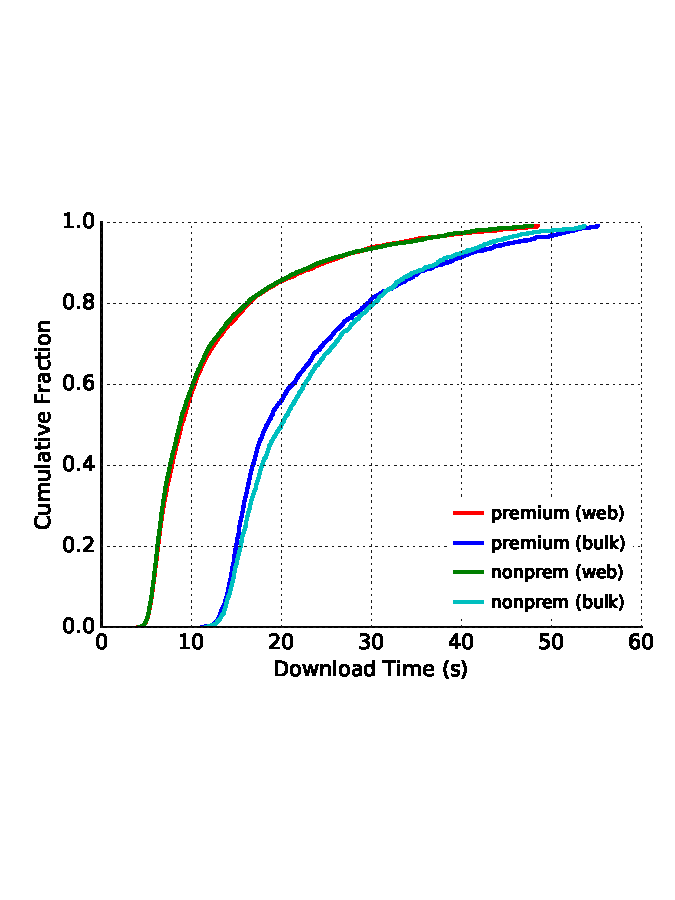
\includegraphics[trim={0 3cm 0 3cm}, clip, width=0.32\textwidth]{images/scheduling_priority.pdf}
  \caption[Prioritized Scheduling]{Prioritized Scheduling --- CDF download
    times for superimposed web and bulk clients where premium status is enforced
    only via scheduling. Almost no priority is observed.}
  \label{fig:scheduling_priority}
\end{figure}

\subsection{Investigation and discussion}

Our negative results can be explained if scheduling is not the most decisive
determining factor in performance. To verify this hypothesis, we studied the
incoming queue from which the scheduler is able to select new active
circuits. Figure~\ref{fig:scheduling_far} illustrates the temporal load in the
queue at a single exit relay over a one-minute time span. The height of the
curve represents the total number of cells waiting to be serviced at each
continuous point in time while the colors group quantities of cells that belong
to the same circuit. Figure~\ref{fig:scheduling_close} displays a subset of the
same information within a smaller time interval.\footnote{While the graph has
  the visual appearance of a bar graph, this is just a function of the striking
  data pattern. In actuality, the plot displays a stacked area graph.} In the
aforementioned figures, notice that the queue is only populated for a period of
10 $ms$ before it is completely flushed, implying the queue spends the vast
majority of its time empty. This 10 $ms$ window is a product of Tor's internal
event handling framework and is consistent with data from Jansen et
al~\cite{jansen2018kist}. We found in an analysis of the line-by-line
observations of the queue activity that while cells are flushed in the correct
order, they appear in the queue at roughly equal proportions. In effect,
bandwidth in our simulation is not constrained by the ordering policy of the
scheduler but rather by the rate at which they arrive from the network. As a
consequence, local decisions at a particular relay for scheduling falls short
to offer the expected priority. Note that the same problem was already spotted by Jansen \textit{et al.}~\cite{jansen2018kist} which motivated the deployment of KIST. Our results show that despite the use of KIST, relays may still be able to flush all queues at once, dismissing the effect of the scheduler's choice. 


\begin{figure} \centering
  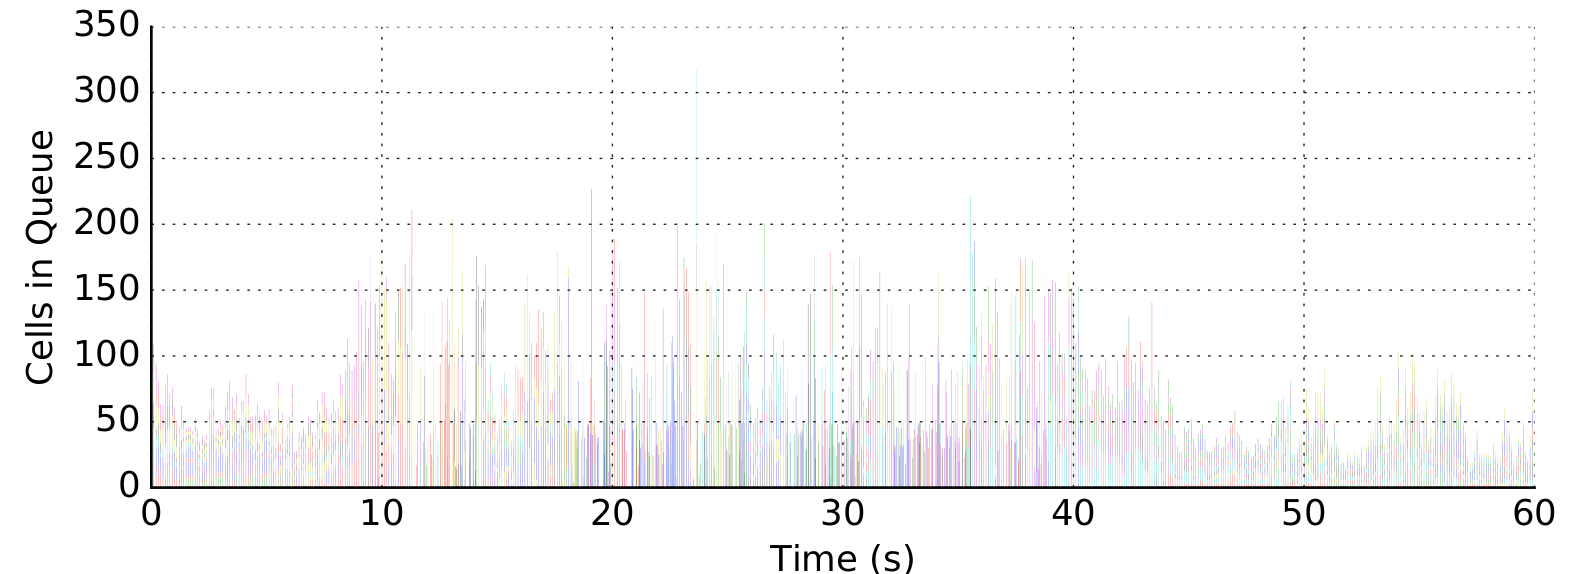
\includegraphics[width=0.49\textwidth]{images/scheduling_far.png}
  \caption[Queue Temporal Profile (60 seconds)]{Queue Temporal Profile
      (60 seconds) --- Size of the scheduling buffer over time at a single exit
    relay in terms of number of cells. Colors group cells belonging to the same circuit.}
  \label{fig:scheduling_far}
\end{figure}

\begin{figure} \centering
  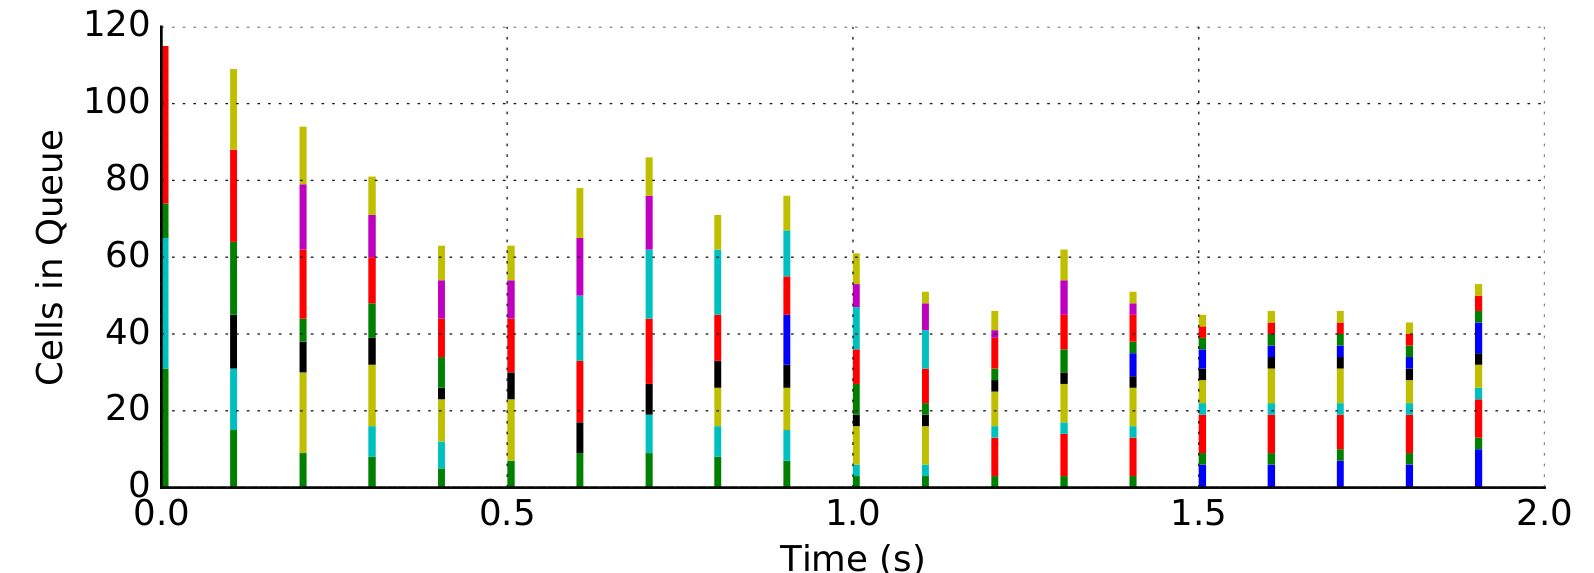
\includegraphics[width=0.49\textwidth]{images/scheduling_close.png}
  \caption[Queue Temporal Profile (2 seconds)]{Queue Temporal Profile
      (2 seconds) --- Size of the scheduling buffer over time at a single exit
    relay in terms of number of cells. Colors group cells belonging to the same
    circuit.}
  \label{fig:scheduling_close}
\end{figure}

Now, we may investigate why this situation happens over our simulations while prioritization based on making decisions inside the 
relay's scheduler worked fine for previous works such as BRAIDS and LIRA while we 
follow the same methodology to evaluate moneTor. So, what could be wrong? First, 
it may be the case
that other network control mechanisms within the Tor codebase constrain the flow
of cells, rendering the mostly idle scheduler to be ineffective. This may be
caused by any combination of factors including point-to-point flow control,
connection throttling, or some less documented threshold embedded in the
code. Yet, we believe that some differences in the code could not explain our 
results for the following reason: our positive results covered in Section~
\ref{sec:priority_exp} showing
increasing performance (resp. decreasing) when we increase (resp. decrease) the 
circuit windows are counter-intuitive compared to previous works exploring the 
effect of changing the window sizes~\cite{archive-2009-mail, kiraly2008solving, 
dingledine2009performance}, and Tor's code covering those aspects did not change 
meaningfully for many years. This is an interesting piece of information, and we 
expect these results to be linked to our actual 
problem of not achieving to prioritize flows based on relays' scheduler decision.

To explain those oddities, we found and verified the following reason: the 
constraining network bottleneck has moved from the
Tor network itself to the exit relay interface with external servers on the
web. In this scenario, cell queuing within Tor is not nearly as important as the
TCP/IP packet handling at each exit relay. Actually, both approaches to prioritize 
flows are complementary: when the congestion is inside the Tor network, applying 
local scheduling policies makes an efficient priority mechanism as demonstrated by previous works. Also in such a situation, priority 
based on the flow-control (that is, a function of the global circuit) would not be 
efficient, because all cells would spend the majority of the time waiting in 
relays' FIFO queues anyway. In the opposite, if the congestion is outside the Tor 
network (between the exit relays and the destination), then local scheduling 
policies would fall short to make any prioritization as showed in Figure~\ref{fig:scheduling_priority}, but priority based on the 
flow-control would achieve to prioritize flows, as demonstrated in Section~\ref{subsec:experiments}. 

The shift of congestion from the internal Tor network to the exit gateways explains why our scheduling results in Figure~\ref{fig:scheduling_priority} are different from BRAIDS
and LIRA. Indeed, BRAIDS run experiments with Tor version \texttt{0.2.0.35} and a network history
from January 2010~\cite{braids-repository}. This Tor version's commit is
before a major change in the path selection mechanism that reduced Tor's
internal congestion problem and greatly improved the performance. This major change
was introduced as the bandwidth-weights in Mike Perry's commit \texttt{0ff86042ac16}
dated from September 2010. The bandwidth-weights are a set of weights specified
in the directory specifications, section 3.8.4~\cite{dirspec}, that aim at
balancing the overall network usage. Those weights are
critical for the network performance, and also for
anonymity~\cite{waterfilling-pets2017, wf_proposal}. Importantly, the benefit
of Mike Perry's bandwidth-weights are proportional to the inequalities between
the overall bandwidth in circuit positions. These inequalities are growing fast for years, as we can observe in Figure~\ref{fig:bw_inequalities}.
%In consequences, compared to BRAIDS's experiments which use a non-balanced path selection and a old internally congested network, our moneTor experiments are no more in a situation
%where we have a lot of internal congestion, and we cannot achieve the same
%priority improvement using a local scheduler at each relay.

\begin{figure}
  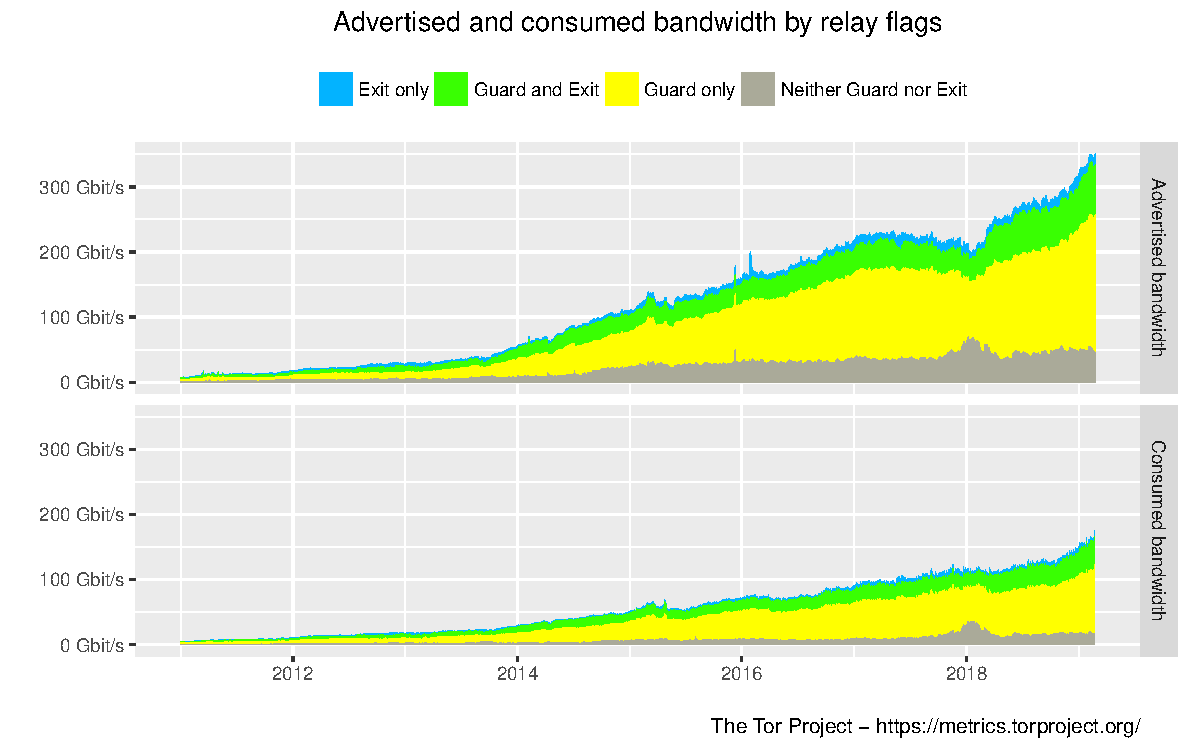
\includegraphics[scale=0.415]{images/bandwidth-flags-2011-01-01-2019-02-25.pdf}
  \caption{Evolution of bandwidth aggregated by relay flags} \label{fig:bw_inequalities}
\end{figure}

LIRA's experiments are based on \texttt{tor-0.2.3.13-alpha} from March 2012, which benefits
from Mike Perry's bandwidth-weights. This may explain why LIRA has less impressive priority advantage than the one exposed in BRAIDS: experiments in LIRA are probably less internally congested than the ones from BRAIDS, and a major change in the path selection to solve a performance problem seems to bear some responsibilities for this case. However, the different congestion status may also be due to other factors, such as a different client usage model and the local scheduling policies. Comparing to our experiments, LIRA uses a simulated environment scaled down from an April 2012 consensus with $\approx 42\%$ of relays with the \texttt{Exit} flag, while our experiments only have $\approx 13\%$ of relays with the \texttt{Exit} flag. This is a consequence of the state of the Tor network from which Shadow simulations are built. The difference in the state of the Tor network may also be observed on Figure~\ref{fig:bw_comp}, where we plotted the distribution of bandwidth allocated to each position. LIRA's experiments were performed when the exit capacity of the Tor network was not scarce. This is not the case anymore as observed for moneTor's used consensus. This result holds now since a few years~\cite{waterfilling-pets2017}.


\begin{figure}
	\centering
  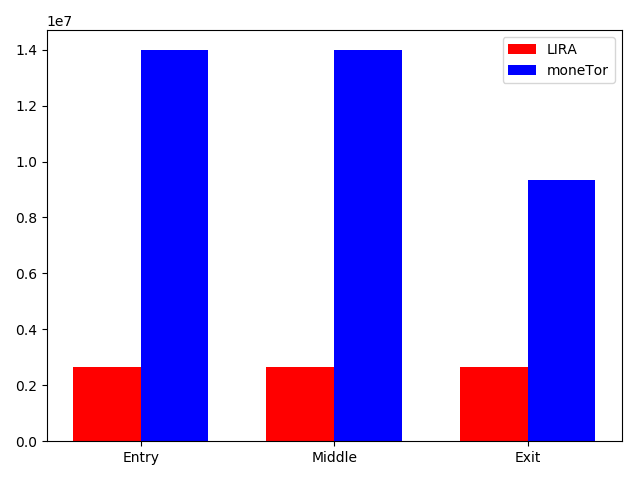
\includegraphics[scale=0.415]{images/bw_analysis_comp.png}
  \caption{Bandwidth distribution in consensuses used for BRAIDS, LIRA and moneTor experiments - BRAIDS does not benefit from bandwidth-weights to refill Middle, LIRA benefits from bandwidth-weights to offer balance between all positions, moneTor benefits from bandwidth-weights to balance entry and middle, yet does not have enough exit nodes to achieve the full balance} 
  \label{fig:bw_comp}
\end{figure}

 
To summarize, as the network grows to offer a lot of internal bandwidth (Figure~\ref{fig:bw_inequalities}, Figure~\ref{fig:bw_comp}), LIRA and BRAIDS's schedulers would tend to become less efficient for providing priority, as demonstrated in our experiments and showed in Figure~\ref{fig:scheduling_close}. 
We must emphasize that we argue for a tendency: our results are no way indicative of the exact same state of affairs for all relays in the real Tor network. The aforementioned experiments
were performed on a considerably smaller scale than the real Tor network with simplistic models for
network topology and user behavior. What can be said is that networking as a
whole is an immensely complex and unpredictable domain and that the attainment
of a simulation environment conducive to effective scheduling is, at the very
least, nontrivial. Consequently, we could argue that the barrier to deploy monetary incentives is not only a social barrier. We may not be ready on a technical level, and technical properties of the scheme may influence social aspects. We showed in this work to be able to offer novel technical properties such as a payment system that scales with trustless entities and fair-exchange (i.e., you pay for what you use), maybe other desirable properties remain to be discovered? Moreover, further research should be conducted to find an ideal priority mechanism that covers various
aspect of circuit congestion. We leave the design of a new priority-based scheme which takes those aspects in account as a further work.

%To confirm it, we run highly congested simulations with many more Tor clients
%than what the scaled-down Tor network could reasonably handle, and observed
%the same results: we were not able to achieve meaningful flow priority with
%local scheduling decisions, but only by tweaking the flow-control mechanism.

%Full paper available at http://u6qr2zmt2bhiw5tm.onion/gender-jubilant, using Tor Browser (total of 21 pages with extensive analysis on why a scheduling-based priority does not work well).
%Full paper available at http://u6qr2zmt2bhiw5tm.onion/gender-jubilant, using Tor Browser (total of 21 pages with extensive analysis on why a scheduling-based priority does not work well).


\end{document}
